% chapter 4

\chapter{Resultados} % chapter title

\label{ch:resultados} % for referencing the chapter elsewhere, use \autoref{ch:mathtest}

%----------------------------------------------------------------------------------------


\section{La importancia del \agn~ en los modelos de formaci\'on de galaxias}
\label{sec:agnoff}

Uno de los desaf\'ios actuales al cual se enfrentan los modelos de formaci\'on de galaxias, en lo que 
respecta a las galaxias masivas, consiste en controlar el excesivo enfriamento del gas para as\'i evitar tasas 
de formaci\'on estelar por encima de los valores que se observan en el universo. En la actualidad, se sabe que los 
c\'alculos efectuados sin incluir una inhibici\'on eficiente sobre el ensamblaje de la masa estelar en el extremo 
masivo de la funci\'on de masa, donde el \textit{feedback} de supernovas se vuelve ineficiente, 
lleva a una sobre predicci\'on de la masa 
estelar en estos sistemas por un factor $\sim$10 (ej, \cite{ben03}). Tales resultados hacen que sea
necesario incluir una fuente adicional de calentamiento del gas. La soluci\'on m\'as
prometente viene de la mano del \textit{feedback} proveniente de las actividad \agn.

%el {\it feedback} de supernovas, utilizado en los modelos para controlar la formaci\'on estelar en galaxias,
%deja de ser eficiente en aquellas m\'as masivas, en particular, en las \bcgs, donde es necesaria
%una fuente adicional de calentamiento 
%para el gas. la soluci\'on m\'as prometente es el {\it feedback} proveniente de la actividad agn.

Sorprendentemente, este proceso f\'isico ha sido ignorando en los c\'alculos presentes en los modelos de formaci\'on de galaxias durante
mucho tiempo. Sin embargo, desde hace aproximadamente una d\'ecada, su uso en modelos semianal\'iticos 
y en simumlaciones num\'ericas hidrodin\'amicas, ha crecido progresivamente 
(\cite{gra04}, \cite{spr05}, \cite{bow06}, \cite{crot06}, \cite{mon07}, \cite{sij07}, \cite{som08}, \cite{fab10},
\cite{mcc10}, \cite{mar12}, \cite{rag13}, \cite{bah17}, \cite{pil17}, Martizzi et al. 2016 )

%Granato et al. 2004; Springel, Di Matteo $\&$ Hernquist 2005; Bower et al. 2006; Croton et al. 2006; Monaco,
%Fontanot $\&$ Taffoni 2007; Sijacki et al. 2007; Somerville et al. 2008; Fabjan et al. 2010; McCarthy et al. 2010;
%Martizzi, Teyssier $\&$ Moore 2012; Ragone-Figueroa et al. 2013; Dubois et al. 2014, Martizzi et al. 2016; Bah\'e et al. 2017;
%Pillepich et al. 2017).

En el campo de las simulaciones num\'ericas, el uso del {\it feedback} de \agn~ reduce la masa estelar de las galaxias \bcgs~
en un factor que var\'ia de 2 a 10 dependiendo del modelo y de la masa de la galaxia considerada (Sijacki et al. 2007; Martizzi 
et al. 2012; Stott et al. 2012; Dubois et al. 2013; Ragone-Figueroa et al. 2013).

A modo de visualizar los efectos producidos por la inclusi\'on de la actividad \agn,
la figura \ref{fig:csfmap} muestra los mapas de brillo superficial obtenidos luego de
correr la simulaci\'on con el modelo
de \agn~ apagado (izquierda)
y encendido (derecha), sobre dos \bcgs, una de ellas
perteneciente a la muestra \cmay~ (paneles superiores) y otra de la muestra \cmen~ 
(paneles inferiores).
Dicha elecci\'on permite dar cuenta de la independencia que tienen los resultados, a grandes rasgos, 
respecto a la masa del c\'umulo que las alberga.  
Es notable que el calentamiento del gas por \textit{feedback} de \agn~ resulta eficiente, 
puesto que las
\bcgs~ de la muestra \agnon~ son menos brillantes en las regiones centrales y menos 
extensas que las correspondientes a la muestra \agnoff.
Los c\'irculos exteriores, de radio \rvc, albergan
al total de la masa de la \bcg~ (bajo las consideraciones del presente trabajo),
mientras que los interiores, de radio \rum, abarcan
la mitad de dicha masa.
Tanto para la \bcg~ de la muestra \cmay~ como para la de la muestra \cmen,
los \rvc~ son mayores cuando el ~\agn~ est\'a apagado, dando factores incrementales 
en tama\~no de 1.34 y 1.14 respectivamente.
Lo contrario sucede con el \rum, cuyo factor es 0.69 para la \bcg~ de
las muestra \cmay~ y 0.57 para la correspondiente a la muestra \cmen. Esto nos permite conlcuir que,
si bien globalmente se forman m\'as estrellas puesto que se obtienen tama\~nos
m\'as grandes, en la regi\'on central el efecto es a\'un mayor. El exceso de formaci\'on 
estelar en dichas regiones es tal
que la mitad de la masa est\'a contenida en \'areas m\'as peque\~nas, generando as\'i 
una mayor compacticidad central.
La figura \ref{fig:csfmbcgmh} muestra el impacto que produce el modelo usado en estas 
simulaciones sobre las masas. 
En dicha figura se exponen las masas (a $z=0$) de las dos \bcgs~ y sus respectivos c\'umulos. 
En ambos casos la disminuci\'on de la masa final al encender el \agn~ en la simulaci\'on es evidente. El factor
incremental obtenido en este trabajo es de 3.5 para la \bcg~ de la muestra \cmay~ y 3.8
para la de la muestra \cmen, superando
a todos los valores de masa calculados, a $z=0$, de la muestra principal bajo el modelo 
de \agn~ encendido.
Tambi\'en puede verse que las masas de los halos sufren una peque\~na variaci\'on de 
un modelo a otro. (\MARU{por qu\'e??????})

\begin{figure}[H]
 \hspace*{-0.5cm}
 \includegraphics[height=7cm, width=9.0cm, trim={0cm 2.1cm 3.3cm 1cm},clip]{../al_final/LR/LR_CSF/nodust/grupo0/mu24/D1/091/bmaps_D1_aperturas.pdf}
 \hspace*{-0.27cm}
 \includegraphics[height=7cm, width=9.0cm, trim={3.2cm 2.1cm 0cm 1cm},clip]{../al_final/LR/LR_minpot3_rmmax/nodust/grupo0/mu24/D1/091/bmaps_D1_aperturas.pdf}
 \\
  \hspace*{-0.5cm}
 \includegraphics[height=8cm, width=9.0cm, trim={0cm 0cm 3.3cm 1.1cm},clip]{../al_final/LR/LR_CSF/nodust/grupo0/mu24/D2/091/bmaps_D2_aperturas.pdf}
 \hspace*{-0.27cm}
 \includegraphics[height=8cm, width=9.0cm, trim={3.2cm 0cm 0cm 1.1cm},clip]{../al_final/LR/LR_minpot3_rmmax/nodust/grupo0/mu24/D2/091/bmaps_D2_aperturas.pdf}
\caption{Mapas de brillos superficiales caracterizados seg\'un la barra vertical de colores.
Gama clara:  $\mu<20$ $mags/arcseg^{2}$.
Gama anaranjada:  $\mu \in [20,21.5)$ $mags/arcseg^{2}$.
Gama lila:  $\mu \in [21.5,24)$ $mags/arcseg^{2}$. 
Lila oscuro:  $\mu \in [24,24.5)$ $mags/arcseg^{2}$.
Gama verde:  $\mu\geq24.5$ $mags/arcseg^{2}$.
Los paneles superiores caracterizan a la
\bcg~ de la muestra \cmay, mientras que los inferiores, representan a la \bcg~ de la muestra \cmen.
A la izquierda se hallan las \bcgs~ \agnoff~ y a la derecha las \agnon}
\label{fig:csfmap}
\end{figure}


\begin{figure}[H]
 \centering
 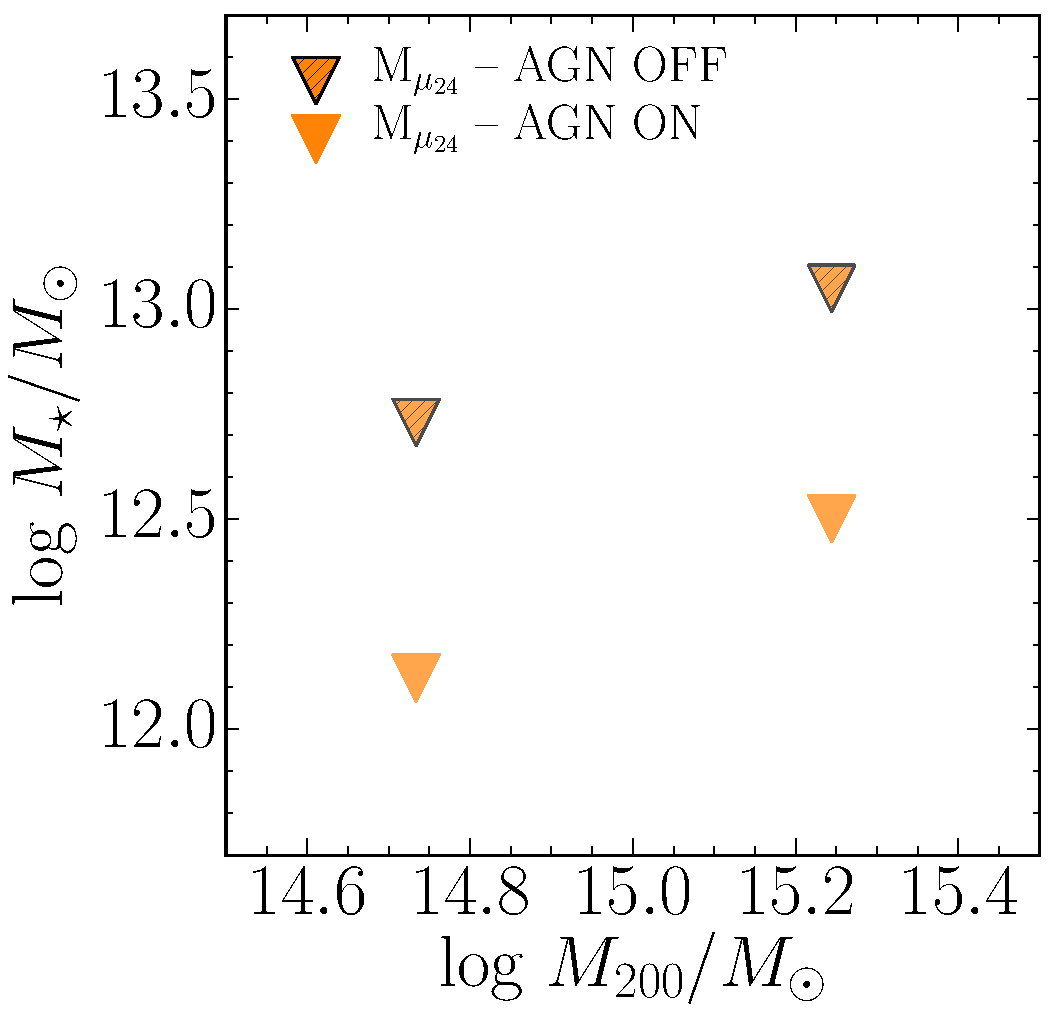
\includegraphics[height=7cm, width=8cm]{../al_final/LR/evolucion/relaciones/csf_agn.pdf}
\caption{Relaci\'on Masa$_{\bcg}$-Masa$_{CUMULO}$. En azul: muestra \agnoff.
En rojo: muestra \agnon.}
\label{fig:csfmbcgmh}
 \end{figure}

\begin{figure}[H]
 \includegraphics[height=7cm, width=8cm]{../al_final/LR/evolucion/relaciones/csf_agn_acumuladas.pdf}
 \includegraphics[height=7cm, width=8cm]{../al_final/LR/evolucion/relaciones/csf_agn_perfil_dens_masa_con_log.pdf}
 \caption{Izquierda: masa acumulada. Derecha: perfil de densisad superficial de masa. Azul: muestra \agnoff. Rojo:  muetsra \agnon. 
 En ambos casos se dintingue la \bcg~ de la muetsra \cmen~ con la
 de la mustra \cmay~ mediante la uni\'on los puntos por una l\'inea continua.}
\label{fig:csfperfiles}
 \end{figure}

Por otro lado, en la figura \ref{fig:csfperfiles} se muestran las distribuciones
de masa acumulada (izquierda) 
y los perfiles de densidad superficial de masa (derecha) para ambos modelos.
En el caso de las masas acumuladas, analizamos separadamente la regi\'on interna ($R\le 42$ kpc)
de la externa ($R\in(42,130]$ kpc). En ambos casos se puede observar que el factor de crecimiento
es mayor en la muestra  \agnon~ que en la muestra \agnoff, aunque siempre predominan
las masas obtenidas en \'esta \'ultima. Las pendientes de crecimiento en la regi\'on interna para
las \bcgs~ de la muestra \agnon~
son $29/41$ $\%$ mayores que las de la muestra \agnoff,
mientras que en la externa son $78/87$ $\%$,
para \bcg-2 y la \bcg-1 respectivamente.
(\MARU{Ser\'a que el agn nos acreta m\'as masa, por sus efectos gravitacionales, es decir, favorece
a las interacciones...???}). En lo que respecta a las densidades superficiales, 
se puede ver que el simple hecho de no considerar los efectos de \agn, produce una
gran compacticidad en la regi\'on interna, donde 
la densidad superficial presenta un decaimiento brusco, efecto que no se visualiza en la muestra
\agnoff, para la cual la variaci\'on de la densidad superficial, en esa misma regi\'on, es
suave.




\section{Masas de la \bcg~ en funci\'on de la apertura}
\label{sec:aperturas}

Como puede verse en la figura \ref{fig:vcmapas}, la gran mayor\'ia de las
\bcgs~ de la muestra \cmay~ a z=0 se muestran con morfolog\'ias m\'as bien
el\'ipticas, por lo cual
necesitamos cuantificar el efecto que produce el uso de
aperturas circulares sobre el c\'alculo de las masas. Para llevar a cabo lo anterior,
se ajustaron elipses a las isofotas caracterizadas
por brillos superficiales $\mu_{v} \in [23.9995,24.0005]$ $mags/arcseg^{2}$, mediante
el uso de la rutina \textit{ellipse} desarrollada
por \textit{Craig B. Markwardt},
sobre el m\'odulo \textit{MPFIT}. Un ejemplo de ajuste 
puede verse en la figura \ref{fig:elipses}, en la cual
se muestra, con una l\'inea amarilla, el ajuste realizado sobre la \bcg-22 y en el
mismo color, las correspondientes
part\'iculas de estrellas que se utilizaron para determinar la masa estelar contenida en el interior
de la elipse, mientras que la l\'inea y puntos lilas, hacen referencia al c\'irculo de radio
\rvc obtenido para esa \bcg~ y las part\'iculas de estrellas
dentro del mismo, pero fuera de la elipse. En este caso, el cociente
entre la masa dentro de la elipse (ME)
y del c\'irculo (MC) es de $\sim$ 1.08, la diferencia representa un $7\%$ de las
part\'iculas estelares contenidas en el c\'irculo, considerando un valor medio de masas
estelares de $\sim 5 \times 10^{7}$M$_{\odot}$.
En t\'erminos generales, todos los ajustes dieron galaxias exc\'entricas, con valores de
excentricidad comprendidos entre 0.55-0.93 y un valor medio de 0.81, sin embargo, como
puede verse en la  figura \ref{fig:distrelcir}, las distribuciones de las masas
MEs y MCs son pr\'acticamente iguales, con un factor entre las medianas dado por,
Med-ME/Med-MC$= 0.93$. 
Esto nos dice que las MCs sobreestiman en un $\sim 7\%$, al valor de las masas MEs.

%la mas excentrica
\begin{figure}[H]
 \centering
 \includegraphics[height=8cm, width=8.8cm]{../al_final/plots/elipses/D22elipse-circ.pdf}
\caption{Visualizaci\'on de la masa contenida dentro del c\'irculo (MC) de radio \rvc~ y
de la elipse (ME) ajustada por la rutina \textit{ellipse}, del m\'odulo \textit{MPFIT},
para la \bcg-22 de la muestra \cmay.
En verde se muestran las part\'iculas del grid, proyectadas sobre el plano XY, con brillos
superficiales: $\mu_{v} \leq 24$ $mags/arcseg^{2}$. 
La l\'inea continua amarilla representa
el resultado del ajuste sobre las part\'iculas antriores, con brillos superficiales: $\mu_{v} \in [23.9995,24.0005]$ $mags/arcseg^{2}$. La 
l\'inea continua lila caracteriza al c\'irculo de radio \rvc. Los puntos lilas y amarillos son part\'iculas de estrellas de la simulaci\'on.}
\label{fig:elipses}
\end{figure}

\begin{figure}[H]
 \centering
 \includegraphics[height=8cm, width=8cm]{../al_final/LR/evolucion/histogramas/Mmu_elipse_vs_circ.pdf}
\caption{Distribuciones de masas a $z=0$, de las \bcgs~ de los c\'umulos principales, dentro de las elipses 
ajustadas por \textit{ellipse} (histograma vac\'io) 
y de los c\'irculos con radios \rvc~ (histograma con rayas diagonales). Las l\'ineas verticales, continua y discontinua,
caracterizan a las medianas de la distribuciones anteriormente mencionadas respectivamente.}
\label{fig:distrelcir}
\end{figure}


\section{\bcgs~ a z=0}
\label{sec:zeta0}

La idea de esta secci\'on radica en exponer las \bcgs~ con las que trabajamos
a z=0 e introducir los \'ordenes de magnitud que se manejan, tanto
en masa como en tama\~nos, de tales galaxias. Con el fin de familiarizarnos
con sus morfolog\'ias, en la figura \ref{fig:vcmapas} se exponen los mapas
de color de las 24 \bcgs~ que integran a la muestra \cmay, en la misma
todos los paneles abarcan 500x500 kpc$^{2}$ y en ellos, las galaxias est\'an delimitadas por el
color m\'as oscuro de lilas, el cual abarca brillos superficiales comprendidos entre
24 -- 24.5 $mags/arcseg^{2}$. A cada una de las \bcgs, tanto de la muestra \cmay, como a
las 5 de la muestra \cmen, se le calcul\'o la masa
seg\'un el m\'etodo descrito en la secci\'on ..., dentro del radio \rvc~ y 
el radio \rum~ que contiene el 50$\%$ de la masa \mvc.
En primera instancia, se muestran en la figura \ref{fig:distrrmuvc}
las distribuciones de radios \rvc para la muestra \cmay~ y \cmen. La distribuci\'on asociada a la 
primera, abarca valores entre
67.8 -- 146.6 kpc con una mediana de 126.9 kpc, mientras que
para la segunda se tienen valores entre 44.2 -- 91.4 kpc, con una mediana de 68.1 kpc.
Posteriormente, en la figura \ref{fig:distrmmuvc} se exhiben las
distribuciones de las masas \mvc contenidas por los c\'irculos de radios \rvc.  
La distribuci\'on asociada a la muestra \cmay~ posee valores comprendidos entre
1 -- 3.8$\times 10^{12}$M$_{\odot}$, con una mediana de 
$2.9\times 10^{12}$M$_{\odot}$, mientras que la asociada a la
muestra \cmen, considera valores de masas entre 
0.3 -- 1.8 $\times 10^{12}$M$_{\odot}$ y est\'a caracterizada por una mediana
de $0.8\times 10^{12}$M$_{\odot}$. Finalmente, en lo que concierne a los radios \rum, la
figura \ref{fig:distrrum} muestra las distribuciones de valores obtenidos de los mismos,
los cuales van de 28.1 a 68.3 kpc para la muestra \cmay, con una mediana de 52.4 kpc,
mientras que la muestra \cmen~ comprende un 
rango de 21.1 -- 39 kpc y su mediana asociada es de 28.5 kpc.


\newpage
\begin{figure}[H] 
\begin{tabular}{c c c c c}
 \hspace*{-1.1cm} \includegraphics[height=3.7cm,width=4cm,trim={3.1cm 2.1cm 4.1cm 1.cm},clip]{../pngs/mapsD1.png}  & 
 \hspace*{-0.3cm}\includegraphics[height=3.7cm,width=4cm,trim={3.1cm 2.1cm 4.1cm 1.cm},clip]{../pngs/mapsD6.png}  & 
 \hspace*{-0.3cm}\includegraphics[height=3.7cm,width=4cm,trim={3.1cm 2.1cm 4.1cm 1.cm},clip]{../pngs/mapsD7.png}  & 
 \hspace*{-0.3cm}\includegraphics[height=3.7cm,width=4cm,trim={3.1cm 2.1cm 4.1cm 1.cm},clip]{../pngs/mapsD8.png}  & 
  \hspace*{-0.3cm}\multirow{6}{*}
  {\includegraphics[height=8cm,width=2.5cm,trim={16.cm 1.cm 0cm 1.cm},clip]{../pngs/mapsD8.png}}
 \\

 \hspace*{-1cm}\includegraphics[height=3.7cm,width=4cm,trim={3.1cm 2.1cm 4.1cm 1.cm},clip]{../pngs/mapsD10.png}  & 
 \hspace*{-.3cm}\includegraphics[height=3.7cm,width=4cm,trim={3.1cm 2.1cm 4.1cm 1.cm},clip]{../pngs/mapsD11.png}  & 
 \hspace*{-.3cm}\includegraphics[height=3.7cm,width=4cm,trim={3.1cm 2.1cm 4.1cm 1.cm},clip]{../pngs/mapsD12.png}  & 
 \hspace*{-.3cm}\includegraphics[height=3.7cm,width=4cm,trim={3.1cm 2.1cm 4.1cm 1.cm},clip]{../pngs/mapsD13.png}  &
 \\

 \hspace*{-1cm}\includegraphics[height=3.7cm,width=4cm,trim={3.1cm 2.1cm 4.1cm 1.cm},clip]{../pngs/mapsD14.png}  & 
 \hspace*{-.3cm}\includegraphics[height=3.7cm,width=4cm,trim={3.1cm 2.1cm 4.1cm 1.cm},clip]{../pngs/mapsD15.png}  & 
 \hspace*{-.3cm}\includegraphics[height=3.7cm,width=4cm,trim={3.1cm 2.1cm 4.1cm 1.cm},clip]{../pngs/mapsD16.png}  & 
 \hspace*{-.3cm}\includegraphics[height=3.7cm,width=4cm,trim={3.1cm 2.1cm 4.1cm 1.cm},clip]{../pngs/mapsD17.png}  &
 \\ 

 \hspace*{-1cm}\includegraphics[height=3.7cm,width=4cm,trim={3.1cm 2.1cm 4.1cm 1.cm},clip]{../pngs/mapsD18.png}  & 
 \hspace*{-.3cm}\includegraphics[height=3.7cm,width=4cm,trim={3.1cm 2.1cm 4.1cm 1.cm},clip]{../pngs/mapsD19.png}  & 
 \hspace*{-.3cm}\includegraphics[height=3.7cm,width=4cm,trim={3.1cm 2.1cm 4.1cm 1.cm},clip]{../pngs/mapsD20.png}  & 
 \hspace*{-.3cm}\includegraphics[height=3.7cm,width=4cm,trim={3.1cm 2.1cm 4.1cm 1.cm},clip]{../pngs/mapsD21.png}  &
 \\ 

 \hspace*{-1cm}\includegraphics[height=3.7cm,width=4cm,trim={3.1cm 2.1cm 4.1cm 1.cm},clip]{../pngs/mapsD22.png}  & 
 \hspace*{-.3cm}\includegraphics[height=3.7cm,width=4cm,trim={3.1cm 2.1cm 4.1cm 1.cm},clip]{../pngs/mapsD23.png}  & 
 \hspace*{-.3cm}\includegraphics[height=3.7cm,width=4cm,trim={3.1cm 2.1cm 4.1cm 1.cm},clip]{../pngs/mapsD24.png}  & 
 \hspace*{-.3cm}\includegraphics[height=3.7cm,width=4cm,trim={3.1cm 2.1cm 4.1cm 1.cm},clip]{../pngs/mapsD25.png}  &
 \\ 

 \hspace*{-1cm}\includegraphics[height=3.7cm,width=4cm,trim={3.1cm 2.1cm 4.1cm 1.cm},clip]{../pngs/mapsD26.png}  & 
 \hspace*{-.3cm}\includegraphics[height=3.7cm,width=4cm,trim={3.1cm 2.1cm 4.1cm 1.cm},clip]{../pngs/mapsD27.png}  & 
 \hspace*{-.3cm}\includegraphics[height=3.7cm,width=4cm,trim={3.1cm 2.1cm 4.1cm 1.cm},clip]{../pngs/mapsD28.png}  & 
 \hspace*{-.3cm}\includegraphics[height=3.7cm,width=4cm,trim={3.1cm 2.1cm 4.1cm 1.cm},clip]{../pngs/mapsD29.png}  &
 \\
\end{tabular}
\caption{Mapas de brillos superficiales de las \bcgs~ pertenecientes a la muestra \cmay.
Cada panel abarca 500x500 kpc$^{2}$.
La barra vertical indica la asignaci\'on de colores seg\'un  el brillo superficial correpondiente.
Gama clara:  $\mu<20$ $mags/arcseg^{2}$. Gama anaranjada:  $\mu \in [20,21.5)$ $mags/arcseg^{2}$.
Gama lila:  $\mu \in [21.5,24)$ $mags/arcseg^{2}$. Lila oscuro:  $\mu \in [24,24.5)$ $mags/arcseg^{2}$.
Gama verde:  $\mu\geq24.5$ $mags/arcseg^{2}$}
\label{fig:vcmapas}
\end{figure}
\newpage

\begin{figure}[H]
 \centering
 \includegraphics[height=8cm, width=8cm]{../al_final/LR/evolucion/histogramas/R24_grandes_chicasz0.pdf}
\caption{Distribuci\'on de radios \rvc~ de las \bcgs~ para la muestra \cmay~ (histograma vac\'io) con su correspondiente 
mediana (l\'inea vertical continua) y para las \bcgs~ de la muestra \cmen~ (histograma con rayas diagonales) con su mediana (l\'inea vertical discontinua)}
\label{fig:distrmmuvc}
\end{figure}

\begin{figure}[H]
 \centering
 \includegraphics[height=8cm, width=8cm]{../al_final/LR/evolucion/histogramas/Mmu_grandes_chicasz0.pdf}
\caption{Lo mismo que en la figura \ref{fig:distrmmuvc}, para los radios \mvc.}
\label{fig:distrrmuvc}
\end{figure}

\begin{figure}[H]
 \centering
 \includegraphics[height=8cm, width=8cm]{../al_final/LR/evolucion/histogramas/R50_grandes_chicasz0.pdf}
\caption{Lo mismo que en la figura \ref{fig:distrmmuvc}, para los radios \rum.}
\label{fig:distrrum}
\end{figure}



\section{Relaciones Masa \bcg-Masa C\'umulo a z=0}
\label{sec:mbcgmcum}

Como se ha mencionado en la introducci\'on, las propiedades de las 
\bcgs~ est\'an fuertemente ligadas al entorno denso
donde les ha tocado evolucionar, por ello se espera encontrar 
correlaciones entre tales propiedades con las
del c\'umulo que las alberga. 

Existe, por ejemplo, un amplio debate en la literatura respecto a la
correlaci\'on entre la masa estelar de la \bcg~ con la masa del c\'umulo,
la cual viene dada por la ley de potencias: M$_{*BCG}=\widetilde{\beta}$M$_{CUMULO}^{\alpha}$.	 
Si bien la tendencia es que para c\'umulos m\'as masivos se obtienen 
\bcgs~ m\'as masivas, en algunos resultados observacionales
la correlaci\'on es d\'ebil (\cite{whi08}), mientras que en otros es un poco m\'as
marcada (\cite{bel16}). 
Tales diferencias pueden deberse a la
gran variedad de t\'ecnicas, mencionadas en la secci\'on ..., para determinar la luminosidad total de la \bcg~ y 
su consecuente masa estelar. En \cite{haa10},
encuentran que los estudios fotom\'etricos basados en aperturas
m\'etricas fijas dan relaciones, entre la masa de la \bcg~ y la del c\'umulo, 
menos pronunciadas que aquellas que se derivan a partir de magnitudes isofotales 
o mediante la extrapolaci\'on del ajuste de alg\'un modelo, ya sea de S\'ersic y/o de de Vaucouleurs,
sobre sus perfiles de luz. Entre los resultados obtenidos a partir del
uso de aperturas e isofotas, se tienen valores para $\alpha$ en el rango 0.11 -- 0.26
(\cite{bro08}, \cite{whi08},
\cite{pop07}, \cite{lin04}), mientras que al implementar la extrapolaci\'on de los ajustes,
se hallan valores m\'as pronunciados, entre 0.62 -- 0.78 (\cite{sto12}, \cite{mit09}, \cite{bai14}, \cite{lid12}).
Por otro lado, en \cite{zha16} se argumenta que el exponente $\alpha$ 
crece con el tama\~no de la apertura sobre la \bcg, dando as\'i correlaciones m\'as
fuertes con las afueras de \'estas galaxias, efecto que puede justificarse mediante el
escenario de crecimiento \textit{inside-out} de las mismas.


El modelo de colapso esf\'erico es ampliamente utilizado para describir el proceso de formaci\'on de los halos
de materia oscura. En este modelo cada halo est\'a caracterizado por una esfera de radio R$_{vir}$,
dentro de la cual la materia se encuentra virializada\footnote{Se usa el t\'ermino virializado para describir sistemas que satisfacen el Teorema de Virial, el cual
establece que, todo sistema en equilibrio o \textit{quasi}-equilibrio
experimenta una relaci\'on bien definida entre la energ\'ia cin\'etica y potencial dada por $V=-2K$}
, con una densidad media equivalente a 200\footnote{Valor
sugerido por algunas simulaciones num\'ericas.} veces la densidad cr\'itica del universo para un dado \textit{redshift}. 
De tal modelo se desprende la forma de caracterizar a la masa de un c\'umulo por M$_{200}$, definida como la masa
contenida dentro del radio R$_{vir}$.
En el presente trabajo se hace uso de la misma para cuantificar las masas de nuestros c\'umulos.
En la figura \ref{fig:relmtmv} se puede ver, en l\'ineas discontinuas, cada una de las relaciones log-log obtenidas a $z=0$,
los datos calculados repesentados por tri\'angulos y en c\'irculos, los datos observacionales de \cite{kra14}.
Entre nuestros datos se dintinguen dos tipos de masas para
cada \bcg, la ya mencionada calculada a partir de la t\'ecnica
descrita en la secci\'on ... en color anaranjado y en verde, una forma alternativa
dada por la masa encerrada en un radio equivalente al 10$\%$ del radio que contiene
500 veces las densidad cr\'itica del universo (\MARU{CITAAAAAAAAAAAAAAAAAAAAAAA}). Es notable
que \'esta \'ultima resulta una buena aproximaci\'on para la cuantificaci\'on de la masa de 
nuestras galaxias, dando ajustes lienales con una pendiente
media de 0.98$\pm$ 0.04, siendo as\'i, pr\'acticamente valores id\'enticos.
Por otro lado, los valores $\alpha$ obtenidos por el presente trabajo
(ver tabla \ref{tab:1}) se encuentran entre los resultados observacionales dados por \cite{lid12}, \cite{bai14}, \cite{bel16},
\cite{sto12}, \cite{mit09}, \cite{zha16}, etc. 


\begin{figure}[H]
 \centering
 \includegraphics[height=8cm, width=8.7cm]{../al_final/LR/evolucion/relaciones/__mtotales2.pdf}
\caption{Relaci\'on Masa$_{\bcg}$-Masa$_{CUMULO}$. Tri\'angulos celestes: masa contenida dentro del 10$\%$ del 
radio que abarca 500 veces la densidad cr\'itica del universo (a $z=0$). Tri\'angulos anaranjados: masas calculadas dentro del
radio de la isofota $\mu_{V}=24$ $mags/arcseg^{2}$. C\'irculos : masas de las \bcgs~ en la muestra 
\cite{kra14}. L\'ineas discontinuas celestes: ajuste lineal log-log para la masa M$_{R<0.1R_{500}}$.
%M$_{R<0.1R_{500}}$/M$_{\odot}$-log M$_{200}$/M$_{\odot}$.
L\'ineas discontinuas anaranjadas: ajuste lineal log-log para la masa \mvc.}
%\mvc~ /M$_{\odot}$-log M$_{200}$/M$_{\odot}$}
\label{fig:relmtmv}
\end{figure}


\begin{table}[H]
\centering
\begin{tabular}{c|c|c c c c}
\hline
& &z=0& z=1& z=2& z=3\\
\hline
 \multirow{2}{*}{M$_{0.1R_{500}}$--M$_{200}$} &$\alpha$ & 0.69 $\pm$ 0.06 & 0.63 $\pm$ 0.06 & 0.6 $\pm$ 0.1  & 0.6 $\pm$ 0.1 \\
                          &$\beta$  & 2$\pm$ 1 & 2.7 $\pm$ 0.9& 3 $\pm$ 2 & 3 $\pm$ 1 \\
\hline
\multirow{2}{*}{M$_{\mu_{24}}$--M$_{200}$} &$\alpha$ & 0.71 $\pm$  0.08 &  0.6 $\pm$ 0.1 & 0.75 $\pm$ 0.09& 0.78 $\pm$ 0.09 \\
                          &$\beta$  & 2 $\pm$ 1 & 3 $\pm$ 1& 1 $\pm$ 1& 1 $\pm$ 1 \\
\hline
\end{tabular}
\caption{ }\label{tab:1}
\end{table}

Con el fin de analizar la dependencia de la correlaci\'on entre la masa
de la \bcg~ con la del c\'umulo, respecto al tama\~no de la apertura utilizada,
se calcularon las masas contenidas en aperturas de radios 30, 50 y 70 kpc tanto
en 3D, como sus proyecciones en 2D. 
Antes de comenzar con el an\'alisis que nos compete, debemos ver qu\'e
tan bien dan las mismas comparadas con
las obtenidas por trabajos observacionales y por otras simulaciones. 
La figura \ref{fig:relmtmv} muestra las masas calculadas en aperturas de
30 kpc seg\'un distintos autores (grises) y las obtenidas por \'este trabajo (celeste).
Los c\'irculos peque\~nos son datos
de la simulaci\'on \textit{IllustrisTNG} (\cite{pil17}), los \'unicos
calculados tridimensionalmente, de las muestras que se exhiben en dicha figura.
Los c\'irculos grandes y hex\'agonos, son resultados observacionales, obtenidos
por \cite{kra14} y \cite{zha16} respectivamente y la l\'inea discontinua
es el ajuste dado por este \'ultimo entre las masas en estudio y la del c\'umulo.
Se puede ver que los resultados obtenidos por el presente trabajo se encuentran entre los observacionales,
mientras que los de la simulaci\'on \textit{IllustrisTNG}, en medianas, dan valores m\'as altos, siendo tales
resultados lo mejor que pueden dar, puesto que de proyectarlos, los valores ser\'ian a\'un mayores.


Respecto a las masas calculadas en aperturas de 50 kpc, la figura \ref{fig:relmcmc} muestra las obtenidas por los
trabajos observacionales de \cite{kra14} y \cite{gon13}, en c\'irculos y cuadrados respectivamente,
mientras que en estrellas se muestran los obtenidos con la simulaci\'on \textit{C-EAGLE} (\cite{bah17}. Los
tri\'angulos celestes, al igaul que en la figura \ref{fig:relmtrmc},son nuestros resultados.
Nuevamente se observa un buen comportamiento de nuestros resultados respecto a los obtenidos
observacionalmente, mientras que los de la simulaci\'on \textit{C-EAGLE} resultan ser superiores.


Siendo entonces, buenas, las aproximaciones obtenidas de las masas dentro de aperturas,
por lo expuesto anteriormente, vale la pena analizar c\'omo dependen \'estas respecto a la masa
del c\'umulo, para ello
se efectuaron ajustes lineales log-log de tales masas respecto a la masa del c\'umulo.
Los resultados obtenidos se exponen en la tabla \ref{tab:2} y, 
en la figura \ref{fig:app} se
muestran los ajustes $\pm1\sigma$. En dicha figura puede verse que la correlaci\'on en ambos casos, 2D y 3D,
se intensifica a medida que se incrementa el tama\~no de la apertura, al igual que en \cite{zha16}.
Tales autores obtienen un factor $\sim 0.12$ entre el \'indice $\alpha$ obtenido para una apertura de 60 kpc
y una de 15 kpc, mientras que en este trabajo se obtiene un factor de $\sim 0.11$ entre
la apertura de mayor y menor tama\~no en 2D y $\sim 0.5$ en 3D.
Esto nos dice que las conclusiones llevadas a cabo por \cite{zha16}
no est\'an afectadas por sesgos observacionales vinculados a la proyecci\'on de la luz,
puesto que, si bien el factor es menor, el comportamiento se mantiene en 3D,
por lo tanto, puede que la masa del c\'umulo correlacione
mejor con las partes m\'as externas de las \bcgs.

\begin{figure}[H]
 \centering
 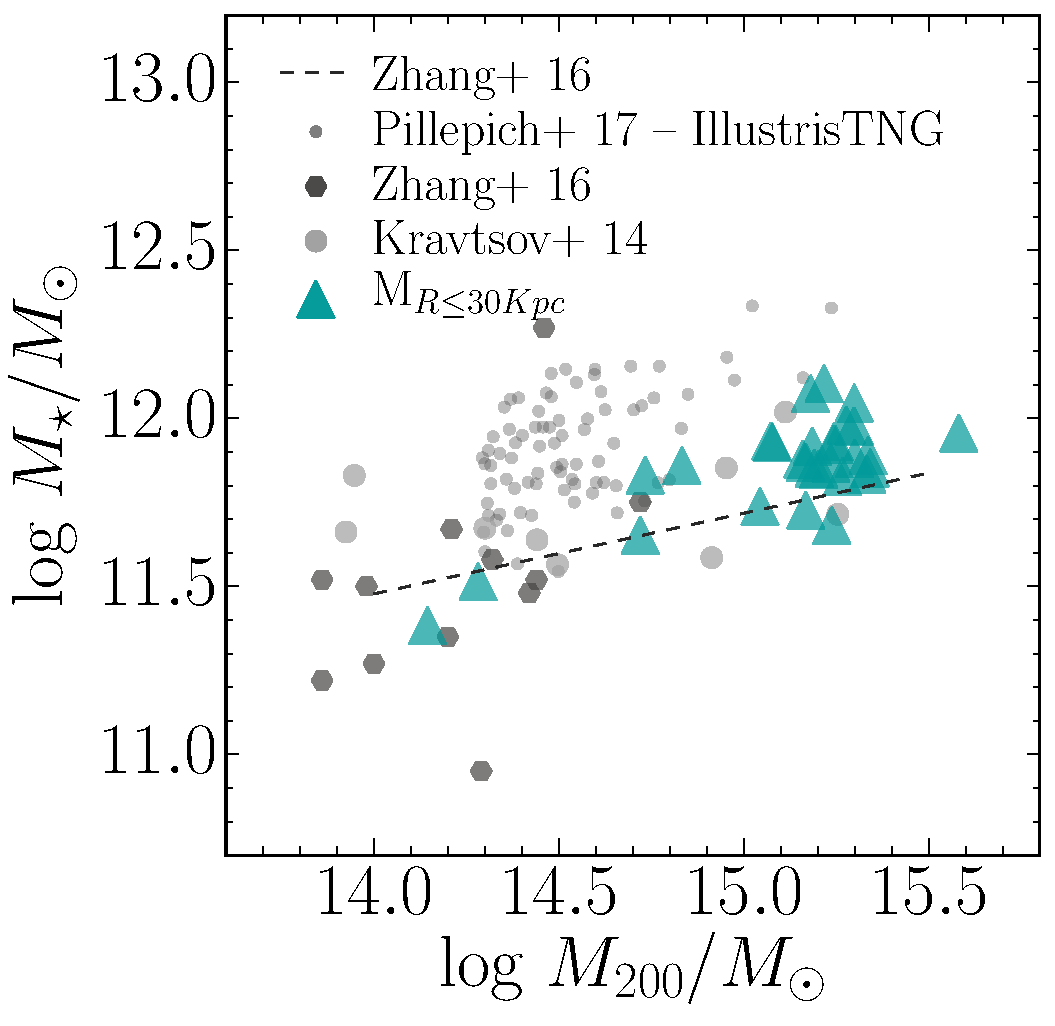
\includegraphics[height=8cm, width=8.7cm]{../al_final/LR/evolucion/relaciones/M302D_vs_M200.pdf}
\caption{Relaci\'on Masa$_{APERTURA}$-Masa$_{CUMULO}$ para aperturas de 30kpc. En tri\'angulos se muestran las masas M$_{R<30kpc-2D}$ calculadas por el presente trabajo.
Los c\'irculos grandes son las masas M$_{R<30kpc-2D}$ de la muetsra Kravtsov+14. Los hex\'agonos representan la masas M$_{R<32kpc-2D}$ de la muestra
Zhang+16. Los c\'irculos peque\~nos caracterizan las masas M$_{R<30kpc-3D}$ de la muestra Pillepich+17. La l\'inea discontinua es 
el ajuste llevado a cabo por Zhang+16
}
\label{fig:relmtrmc}
\end{figure}


\begin{figure}[H]
 \centering
 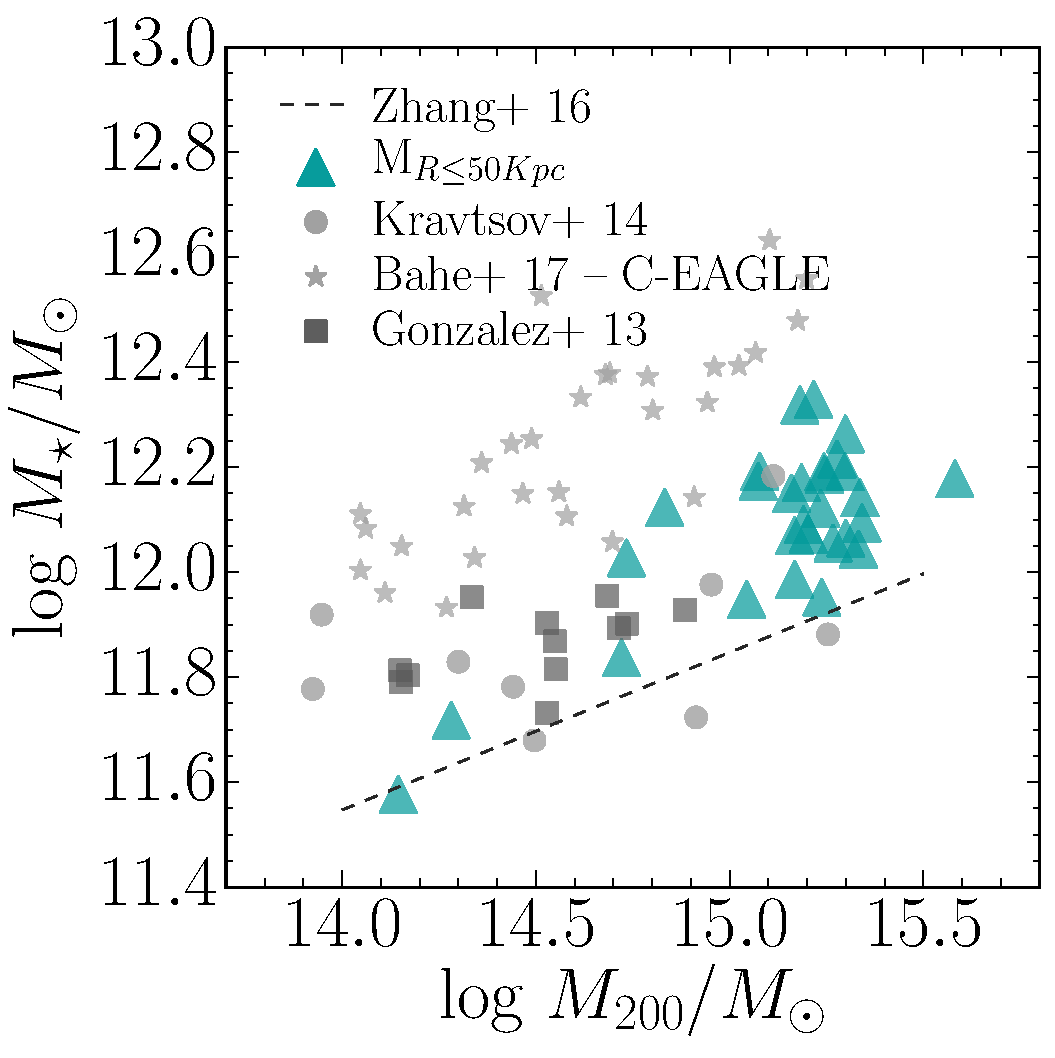
\includegraphics[height=8cm, width=8.7cm]{../al_final/LR/evolucion/relaciones/M502D_vs_M200.pdf}
\caption{Relaci\'on Masa$_{APERTURA}$-Masa$_{CUMULO}$ para aperturas de 50kpc. Los tri\'angulos son las masas M$_{R<50kpc-2D}$ calculadas por el presente trabajo.
Los c\'irculos representan a las masas M$_{R<5kpc-2D}$ de la muestra Kravtov+14. Las estrellas caracterizan a las masas M$_{R<50kpc-2D}$ de la muestra Bah\'e+17.
Los cuadrados son las masas M$_{R<50kpc-2D}$ de la muestra Gonzalez+13.}
\label{fig:relmcmc}
\end{figure}




\begin{figure}[H]
 \centering
 \includegraphics[height=8cm, width=8.7cm]{../al_final/LR/evolucion/relaciones/ajustesaperturas.pdf}
\caption{Ajustes lineales de la relaci\'on Masa$_{APERTURA}$-Masa$_{CUMULO}$ para aperturas de 30
50 y 70 kpc (violeta, verde y rojo, respectivamente), para masas pryectadas (2D, l\'ineas discontinuas)
y no proyectadas (3D, l\'ineas continuas.)
}
\label{fig:app}
\end{figure}

\begin{table}[H]
\centering
\begin{tabular}{c|c|c c c}
\hline
& &2D&& 3D\\
\hline
\multirow{2}{*}{M$_{R<30kpc}$--M$_{200}$} &$\alpha$ & 0.38 $\pm$ 0.06  && 0.30 $\pm$ 0.05 \\
                                          &$\beta$  & 6$\pm$ 1         && 7 $\pm$ 1   \\
\hline
\multirow{2}{*}{M$_{R<50kpc}$--M$_{200}$} &$\alpha$ & 0.41 $\pm$  0.07 &&  0.33 $\pm$ 0.06 \\
                                          &$\beta$  & 6 $\pm$ 1        &&  7 $\pm$ 1\\
\hline
\multirow{2}{*}{M$_{R<70kpc}$--M$_{200}$} &$\alpha$ & 0.49 $\pm$  0.07 &&  0.35 $\pm$ 0.06 \\
                                          &$\beta$  & 5 $\pm$ 1        && 7 $\pm$ 1\\
\hline
\end{tabular}
\caption{Par\'ametros $\alpha$ y $\beta$ para las relaciones entre las masas centrales dentro de 
aperturas de 30, 50 y 70 kpc, proyectadas y no proyectadas respecto a la masa del c\'umulo.}\label{tab:2}
\end{table}


\section{Masas de las \bcgs~ a distintos z}
\label{sec:variosz}

En la secci\'on anterior estudiamos el comportamiento, a z=0,
de distintas tipos de masas que pueden asociarse con la \bcg.
Comencemos entonces a 
adentramos en el tema principal del presente trabajo, la evoluci\'on
de la masa de la \bcg. Si bien hemos notado que las aperturas juegan un 
rol importante en lo que concierne a la relaci\'on que existe entre la
masa de estas galaxias con la de su correpondiente c\'umulo, afianz\'andose 
a medida que se toman aperturas m\'as grandes, 
las mejores correlaciones obtenidas fueron para las masas \mvc~ y la M$_{0.1R_{500}}$.
Por tal motivo, nos basaremos en \'estas para estudiar la evoluci\'on de las mismas y comparar con otros
resultados. 
En primer lugar se estudia si tales masas matenienen el v\'inculo
obtenido a z=0, pero en \textit{redshifts} m\'as grandes y se analiza c\'omo evoluciona la relaci\'on
entre cada una de \'estas con la masa del c\'umulo. Dicho estudio abarcar\'a
a los \'ultimos $\sim11.6$ Gyrs del Universo. La figura \ref{fig:mbcgm10} nos muestra,
para los \z~ en estudio, que la relaci\'on entre las masas que caracterizan
a las \bcgs~ va mutando con el tiempo, no mantiene el v\'inculo que se obtuvo a z=0, siendo
las razones entre los valores medios de \mvc/M$_{0.1R_{500}}$,  2, 0.73, 1.25 y 2.55 a z= 0, 1, 2 y 3 respectivamente.
Por otro lado, la relaci\'on log-log a distintos \z~ (ver tabla \ref{tab:1}) resulta
m\'as fuerte para \mvc~ en z= 0, 2 y 3 y creciente entre los mismos. Sin embargo, 
en z=1 se rompe lo anterior, lo cual puede ser atribuido a cuestiones evolutivas, por ejemplo fusiones.


\begin{figure}[H]
\centering
\hspace*{-1.5cm}
 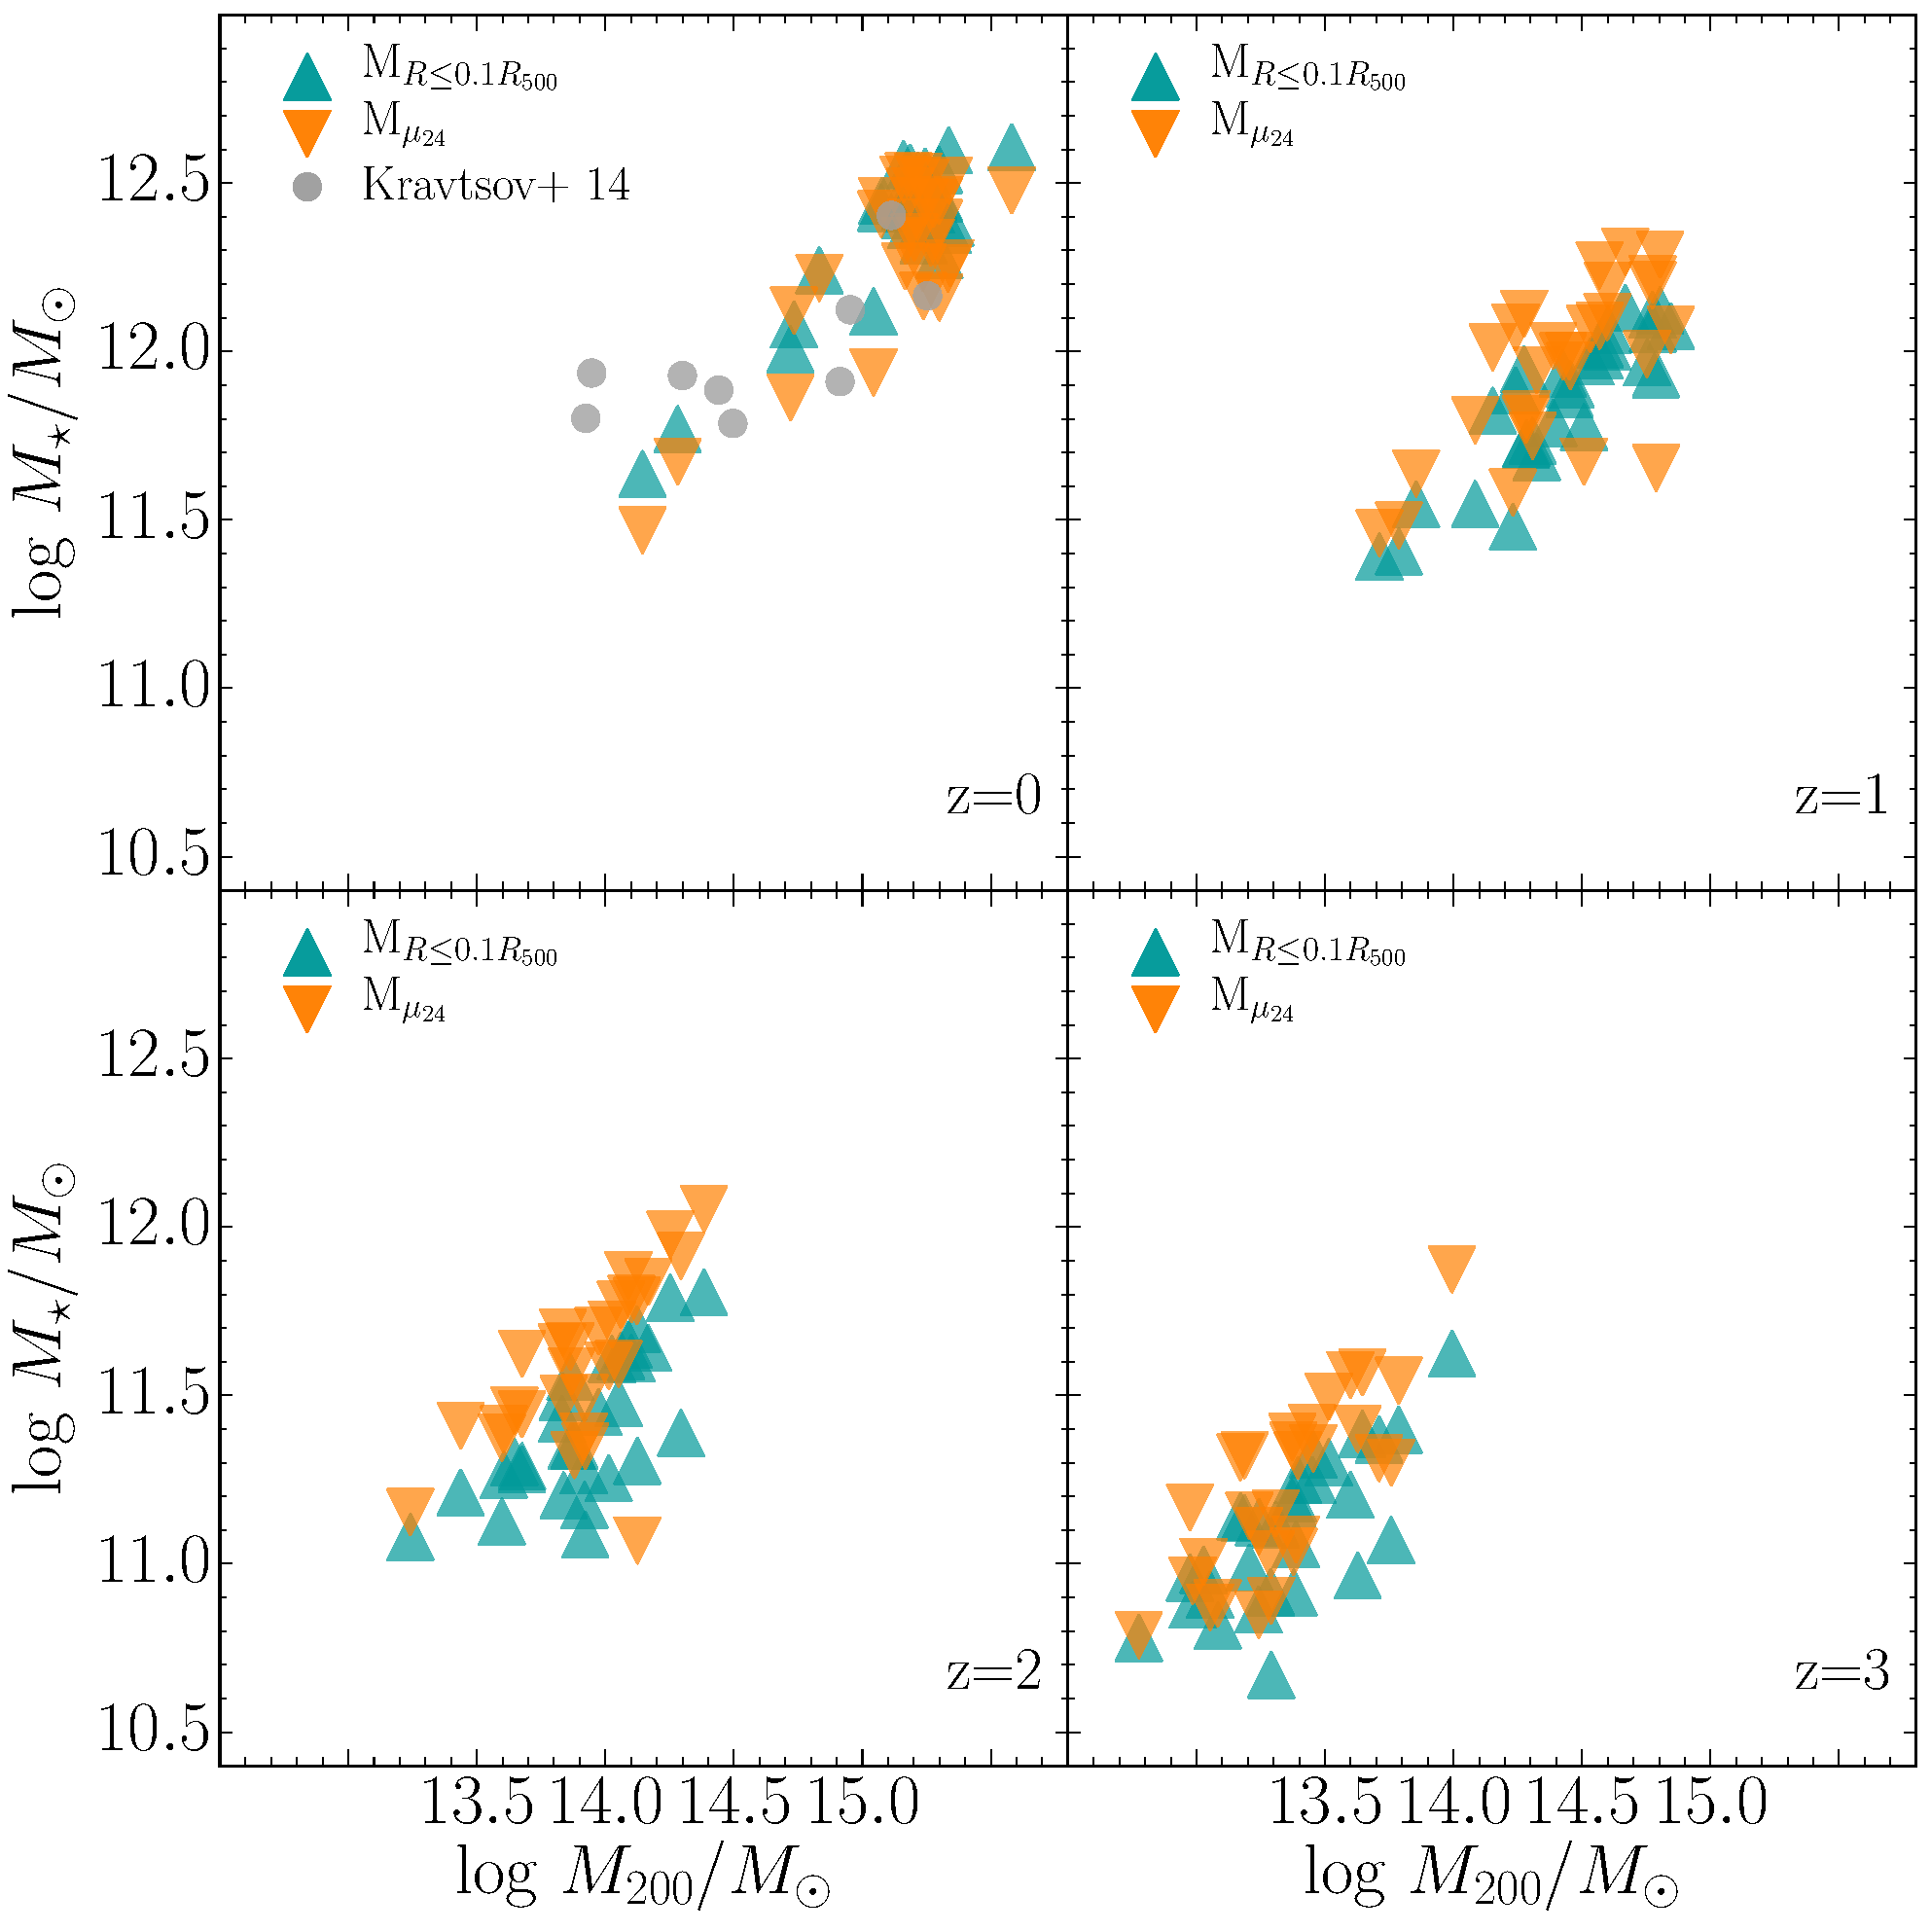
\includegraphics[height=12cm, width=13cm]{../al_final/LR/evolucion/relaciones/muvs10r.pdf}
\caption{Comportamiento de las masas, \mvc~ (tri\'angulos anaranjados) y M$_{R<0.1R_{500}}$ 
(tri\'angulos celestes), respecto a la masa del c\'umulo, para z=0 (arriba, izquierda),
z=1 (arriba, derecha), z=2 (abajo, izquierda), z=3 (abajo, derecha). C\'irculos:  masas de las \bcgs~ en la muestra 
Kravtsov +2014}
\label{fig:mbcgm10}
\end{figure}

\begin{figure}[H]
\centering
\hspace*{-1cm}
 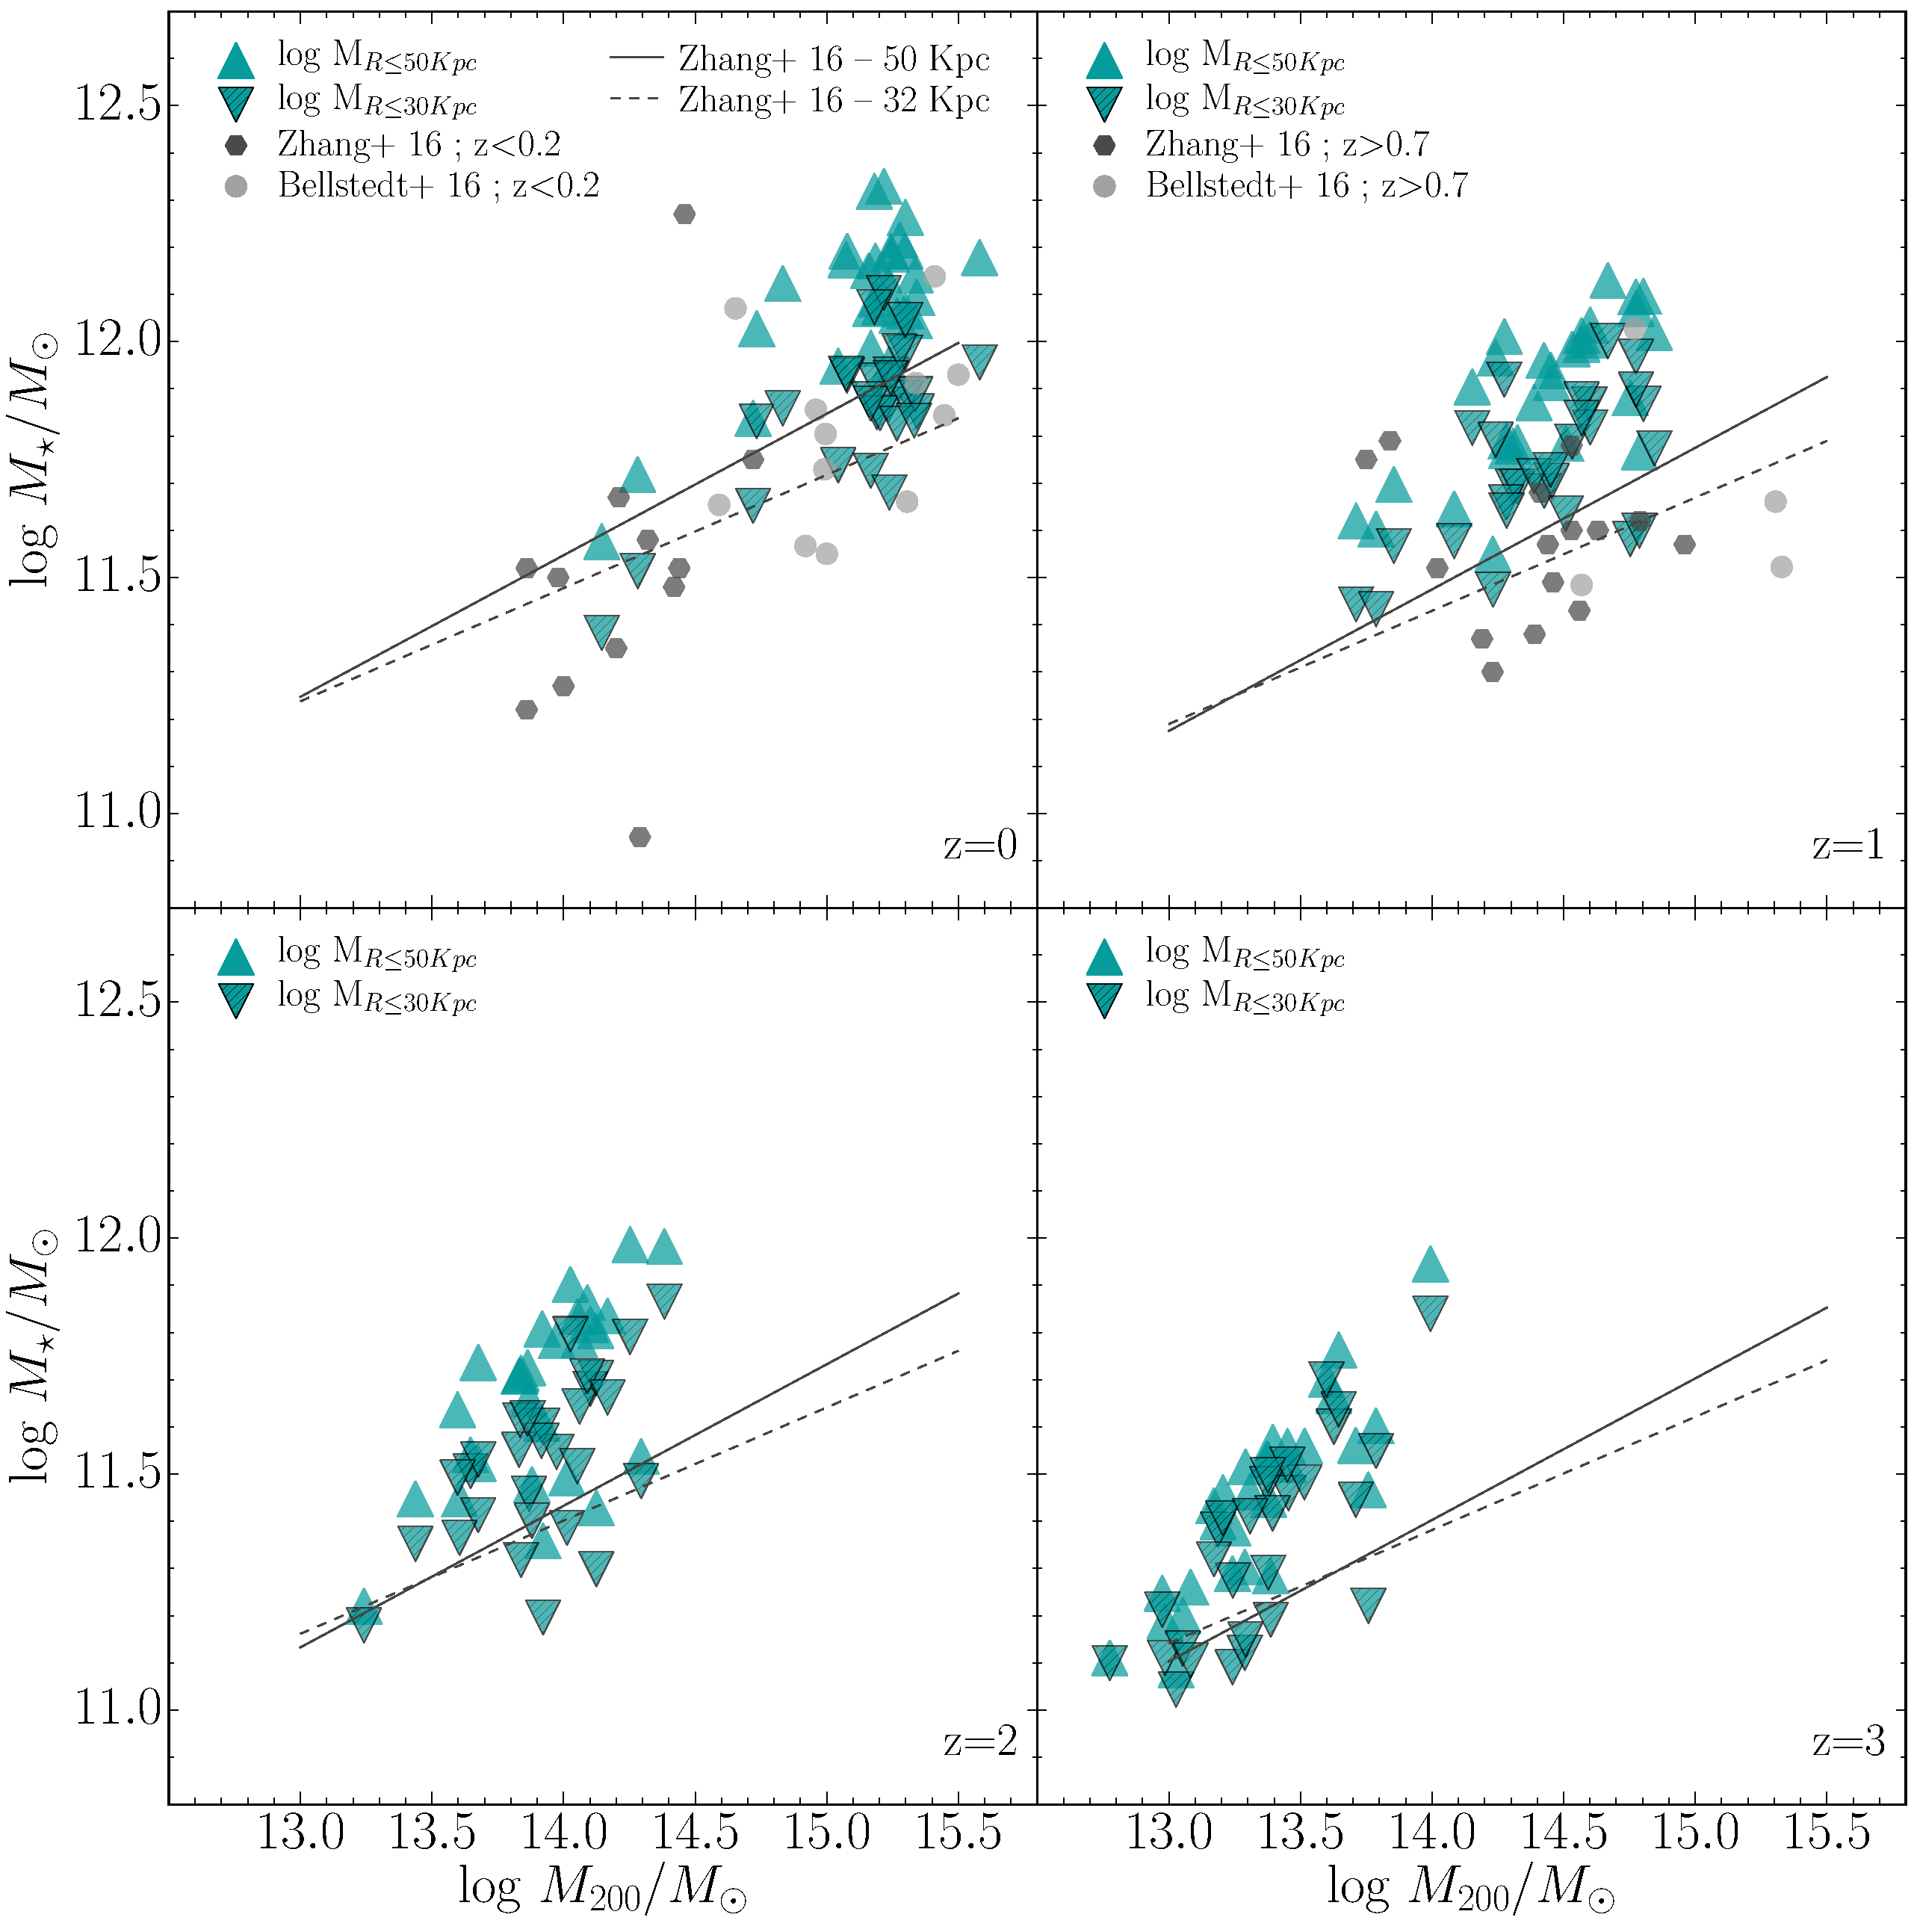
\includegraphics[height=12cm, width=13cm]{../al_final/LR/evolucion/relaciones/zhang_vs_z.pdf}
\caption{Comportamiento de la masa contenida dentro de aperturas circulares de radios R=30kpc (tri\'angulos rayados) y
R=50kpc (tri\'angulos sin rayas) para $z=0$ (arriba, izquierda), $z=1$ (arriba, derecha), $z=2$ (abajo, izquierda) y z=3 (abajo, derecha).
L\'inea discontinua y continua: ajuste en funci\'on de z (Zhang+16) sobre la relaci\'on M$_{R<X}$-M$_{200}$ para aperturas circulares de radios X=32kpc y X=50kpc, respectivamente. 
}
\label{fig:zhang}
\end{figure}

ver: there is also a (weak) correlation between bcg mass and the mass of their host clusters, which does not change significantly
with redshift out to $z\sim 0.8$ (edge 1991; collins $\&$ mann 1998; burke, collins $\&$ mann 2000; brough et al. 2007; stott et al. 2008;
whiley et al. 2008).

\section{Evoluci\'on en Masa}
\label{sec:evolmasa}
Si bien en la secci\'on \ref{sec:tformyevol} se introdujeron
los procesos que hoy se creen pilares para la formaci\'on
y evoluci\'on de las \bcgs~ y 
se coment\'o el modelo de dos fases 
que actualmente se le adjudica a las mismas,
la realidad est\'a lejos ser esclarecedora. Las inmensas contradicciones
existentes entre los resultados observacionales y num\'ericos, evidencian
la falta de entendimiento sobre los mecanismos involucrados en la evoluci\'on
de \'estas, aunque no s\'olo se tienen resultados contradictorios entre los factores
de crecimiento, tambi\'en
se fracasa en el establecimiento de la \'epoca en la que se ensamblan y en los procesos
principales involucrados sobre su evoluci\'on tard\'ia. Por ejemplo, algunos observacionales conlcuyen que desde la mitad
de la edad del universo hasta hoy, las \bcgs~ han aumentado su masa principalmente por fusiones menores no disipativas, mientras
otros dan protagonismo a las fusiones mayores del mismo tipo, no obstante, est\'an los que establecen que deben involucrarse las 
fusiones disipativas y en el otro extremo, los que excluyen todo tipo de fusi\'on. Las mismas
contradicciones se encuentran en las conlusiones llevadas a cabo por estudios te\'oricos.
Entre los diferentes resultados observacionales se encuentran los que muestran poca o no evoluci\'on de la masa estelar
desde $z=1$ hasta hoy (\cite{whi08}, \cite{col09}, \cite{sto10})
y los que obtienen factores de crecimiento cercanos a 2, en ese mismo intervalo
de \z~ (\cite{ara98}). \cite{bur00} justifican que las contradicciones pueden 
deberse al sesgo que existe al seleccionar los c\'umulos progenitores, problema denominado \textit{bias-problem}.
\cite{lid12} y \cite{bai14}, teniendo en cuenta
el problema anterior, encuentran factores de crecimiento $\sim2$ desde $z=1$, $\sim1.5$ desde $z=0.5$, respectivamente.
Por otro lado, entre los primeros estudios te\'oricos
basados en la cosmolog\'ia actualemte aceptada,
se halla el de \cite{del07}, quienes predicen que el contenido estelar de las \bcgs~
se cuadruplic\'o desde $z=1$ hasta hoy principalmente por fusiones menores, mientras que
\cite{lap13} predicen un factor 2 para dicho crecimiento y concluyen que las fusiones
mayores tambi\'en contribuyen sobre tal evoluci\'on.
\cite{gro17} explica que las discrepancias entre los factores observacionales con los num\'ericos,
son aparentes y que puede deberse a que las fusiones no aportan al crecimiento
de las masas de las \bcgs~ si una proporci\'on significativa de la masa termina en la \icl.
Esto \'ultimo nos dice que la formaci\'on y evoluci\'on de la \bcg~ y la \icl~ dentro del c\'umulo,
est\'an \'intimamente conectadas, lo cual se analizar\'a en la secci\'ion ....


La evoluci\'on de la \bcg~ no s\'olo se estudia a partir del crecimiento de su masa. Como
hemos mencionado, los procesos evolutivos alteran la forma en que se distribuye la masa, por ende, es necesario
llevar a cabo un an\'alisis de c\'omo cambia el tama\~no y la concentraci\'on.
En lo que sigue veremos c\'omo han evolucionado las masas
\mvc~ y \mdiez, y los radios \rvc~ y \rum, desde $z=3$, haciendo
distinci\'on entre las muestras
\cmay~ y \cmen.
La forma en la que se han seleccionado las \bcgs~ en cada \textit{redshift}, simula
el procedimiento implementado por la mayor\'ia de los observacionales,
esto es, se escogen las que se hallan en los c\'umulos m\'as masivos, de todos modos, vale la aclaraci\'on,
no necesariamente son las progenitoras de la \bcgs~ a $z=0$.
Las figuras \ref{fig:evolmbcg} y \ref{fig:evolm10} exponen la evoluci\'on de las masas \mvc~ y \mdiez~ respectivamente,
en ambas es notable un crecimiento continuo de las medianas de los valores
obtenidos para cada \textit{redshift} (tabla \ref{tab:medianas}).
Analizando los resultados (tabla \ref{tab:factoresdc}), se observa respecto
a la masa de la \bcg~ dada por \mvc~ que
el factor de crecimiento entre \z~ consecutivos
se mantiene aproximadamente constante para
la muestra \cmay~ y su valor 
se halla entre los encontrados en la literatura,
$\sim2$, mientras que en la muestra 
\cmen~ fluct\'ua entre $1.5$ y $3$.
En cambio para la masa \mdiez,
los factores crecen de un \textit{redshift} 
a otro, lo cual es esperable para un l\'imite que depende de
la evoluc\'on del radio virial de un c\'umulo.

Las figuras \ref{fig:evolr24} y \ref{fig:evolrum} 
muestran c\'omo han evolucionado
los tama\~nos y concentraciones respectivamente.
Comparando las medianas de \rvc~ con \rum~ para cada
\textit{redshift} (tabla \ref{tab:medianas}), la mitad de la masa est\'a contenida dentro
de un 16/29/33/40 $\%$ del
tama\~no de la galaxia, a z = 3, 2, 1 y 0 respectivamente, para
la muestra \cmay~ y un 23/23/34/42 $\%$ para la muestra \cmen.
Estos porcentajes hacen notar que la masa a altos \textit{redshifts}
estaba muy concentrada y con el transcurso del tiempo
esa propiedad se ha ido modificando, lo cual
es esperable para el crecimiento jer\'arquico de las
estructuras. Si bien en la literatura se establece
que el tama\~no, caracterizado por el radio efectivo,
se cuadruplica desde z=1 al presente, en este trabajo
ello no sucede (tabla \ref{tab:factoresdc}).
La figura \ref{fig:factores},
muestra los factores de crecimiento desde z=1 a z=0, tanto de la masa
de la \bcg~ como de \rum, pero s\'olo para aquellas \bcgs que sabemos
sus progenitores a z=1 se hallan en el c\'umulo
m\'as masivo. Los factores esperados son
2 y 4 respectivamente, mientras que en el presente
trabajo los valores medios obtenidos son $\sim2$, $\sim1.5$
respectivamente.

\begin{figure}[H]
 \centering
 \includegraphics[height=7cm, width=14cm]{../al_final/LR/evolucion/observacional/evolucion_M24.pdf}
\caption{Evoluci\'on de la masa \mvc desde $z=3$ a $z=0$. En ambos paneles (\cmay, izquierda y \cmen, derecha), los puntos representan
a la mediana de las masas para cada z, mientras
que la regi\'on rayada est\'a delimitada por el valor m\'inimo y m\'aximo del z correspondiente. 
}
\label{fig:evolmbcg}
\end{figure}

\begin{figure}[H]
 \centering
 \includegraphics[height=7cm, width=14cm]{../al_final/LR/evolucion/simulacion/evolucion_M10_grandes_chicas.pdf}
\caption{Idem que figura \ref{fig:evolmbcg}, para la masa M$_{R<0.1R_{500}}$.}
\label{fig:evolm10}
\end{figure}


\begin{figure}[H]
 \centering
 \includegraphics[height=7cm, width=14cm]{../al_final/LR/evolucion/observacional/evolucion_R24.pdf}
\caption{Idem que figura \ref{fig:evolmbcg}, para el radio \rvc.}
\label{fig:evolr24}
\end{figure}

\begin{figure}[H]
 \centering
 \includegraphics[height=7cm, width=14cm]{../al_final/LR/evolucion/observacional/evolucion_Re.pdf}
\caption{Idem que figura \ref{fig:evolmbcg}, para el radio \rum.}
\label{fig:evolrum}
\end{figure}

\begin{figure}[H]
 \centering
 %\includegraphics[height=7cm, width=7cm]{../al_final/lr/evolucion/histogramas/cocoientesmr24.pdf}
 \includegraphics[height=8cm, width=8cm]{../al_final/LR/evolucion/histogramas/bcocoientesmr1medio.pdf}
 %\\
 %\includegraphics[height=7cm, width=7cm]{../al_final/lr/evolucion/histogramas/cocoientesm30r1medio}
 %\includegraphics[height=7cm, width=7cm]{../al_final/lr/evolucion/histogramas/cocoientesm50r1medio}
\caption{Distribuciones del factor de crecimiento desde $z=1$ a $z=0$ 
para las \bcgs~ de los c\'umulos principales. Histograma con rayas diagonales: factores de creciemiento del tama\~no \rum.
Histograma vac\'io: factores de crecimiento de la masa \mvc.}
\label{fig:factores}
\end{figure}



\begin{table}[H]
\caption{Evoluci\'on desde $z=3$ a $z=0$,
de las masas \mvc~ y \mdiez~ [$\times10^{12}$ M$_{\odot}$],
y los radios \rvc~ y \rum~ [kpcs].}\label{tab:medianas}
\centering
\begin{tabular}{c|c c c c| c c c c}
\hline
 & \multicolumn{4}{c|}{\cmay} &\multicolumn{4}{c}{\cmen}\\
\hline
z&\mvc&\mdiez&\rvc&\rum &\mvc&\mdiez&\rvc&\rum \\
\hline
3& 0.2418 &0.1356 & 54.40  & 8.55   & 0.1047 & 0.0908 & 26.52 & 6.06  \\
2& 0.5594 &0.2757 & 100.50 & 28.66  & 0.2900 & 0.1625 & 59.05 & 13.53 \\
1& 1.2617 &0.8731 & 107.22 & 35.42  & 0.4556 & 0.3518 & 61.75 & 20.81 \\
0& 2.8916 &2.7857 & 127.35 & 50.33  & 0.8325 & 1.0161 & 68.11 & 28.53 \\

\end{tabular}
\end{table}

\begin{table}[H]
\caption{Factores de crecimiento}\label{tab:factoresdc}
\centering
\begin{tabular}{c|c c c c| c c c c}
\hline
 & \multicolumn{4}{c|}{\cmay} &\multicolumn{4}{c}{\cmen}\\
\hline
$\Delta z$ & $f_\mvc$ & $f_\mdiez$ & $f_\rvc$ & $f_\rum$ & $f_\mvc$ & $f_\mdiez$ & $f_\rvc$ & $f_\rum$ \\
\hline
$3-2$& 2.31 & 2.03 & 1.85 & 3.35 & 2.77 & 1.79 & 2.23 & 2.23\\
$2-1$& 2.26 & 3.17 & 1.07 & 1.24 & 1.57 & 2.17 & 1.05 & 1.54\\
$1-0$& 2.29 & 3.19 & 1.19 & 1.42 & 1.83 & 2.89 & 1.10 & 1.37\\
\end{tabular}
\end{table}

Tambi\'en podemos estudiar c\'omo los distintos procesos involucrados
en la evoluci\'on de las \bcgs, modifican las masas contenidas dentro 
de aperturas fijas, para ello, en la figura \ref{fig:evosim} se muestra
la evoluci\'on de tales masas, dentro de aperturas de radios 30, 50 y 70 kpcs,
proyectadas (derecha) y no proyectdas (izquierda), esto \'ultimo, para analizar
la implicancia que tiene la proyecci\'on
en los resultados observacionales. En las tablas \ref{tab:medianasap} y \ref{tab:factoresdcap}
se exponen las medianas obtenidas para cada \textit{redshift} y los factores de crecimiento,
respectivamente.


\begin{figure}[H]
 \centering
 \includegraphics[height=18cm, width=14cm]{../al_final/LR/evolucion/simulacion/evolucion.pdf}
\caption{Evoluci\'on desde $z=3$ a $z=0$, de la masa proyectada 
(derecha, l\'inea discontinua) y no proyectada (izquierda, l\'inea continua), 
contenida dentro de aperturas de radio R=30kpc
(arriba), R=50kpc (centro) y R=70kpc (abajo). En todos lo casos, los puntos representan a 
la mediana (considerando todas las \bcgs~ de los c\'umulos principales) para un dado z,
mientras que la regiones rayadas est\'an delimitadas por los valores m\'aximo y m\'inimo de cada z.}
\label{fig:evosim}
\end{figure}


Es notable que, dentro de los factores de crecimiento, el m\'as grande para un dado
\textit{redshift} es el factor
asociado a la apertura de 70 kpcs,
lo cual implica que la \bcg~ ha ido incrementando su masa
en mayor proporci\'on en las afueras de la misma, ya sea por la 
acreci\'on de la masa de sus sat\'elites mediante interacciones y fusiones,
o por el desplazamiento del material bari\'onico central 
hacia las afueras mediante alg\'un mecanismo de crecimiento adiab\'atico dado
por procesos de \textit{feedback} (\cite{asc11}).
%Esto nos conduce a analizar qu\'e sucede con los
%perfiles de luz y de densidad de masa, c\'omo han evolucionado. para as\'i
%poder inferir si las \bcgs~ responden al crecimiento \textit{inside-out}
%en el cual, la regi\'on central de la galaxia se ha formado primero y su posterior crecieminto se ha dado
%principalmente en las afueras. Te\'oricamente, se espera que las fusiones menores incrementen el tama\~no en las
%afueras de la galaxia, sin alterar la densidad central de la misma.

\begin{table}[H]
\caption{Evoluci\'on desde $z=3$ a $z=0$,
de las masas 2D y 3D 
\mtre, \mcin~ y \mset~
[$\times10^{12}$ M$_{\odot}$].}\label{tab:medianasap}
\centering
\begin{tabular}{c|c c c |c c c}
\hline
 & \multicolumn{3}{c|}{3D} &\multicolumn{3}{c}{2D}\\
\hline
z&\mtre&\mcin&\mset &\mtre&\mcin&\mset\\
\hline
3& 0.1719 & 0.2672 & 0.2898 & 0.2411 & 0.2897 & 0.2897 \\
2& 0.2366 & 0.4322 & 0.5354 & 0.3395 & 0.5112 & 0.5360 \\
1& 0.3557 & 0.6182 & 0.8526 & 0.5193 & 0.8175 & 0.8772 \\
0& 0.4722 & 0.8740 & 1.2369 & 0.7390 & 1.3214 & 1.7384 \\

\end{tabular}
\end{table}

\begin{table}[H]
\caption{Factores de crecimiento de las masas 2D y 3D dentro de
aperturas.}\label{tab:factoresdcap}
\centering
\begin{tabular}{c|c c c |c c c}
\hline
 & \multicolumn{3}{c|}{3D} &\multicolumn{3}{c}{2D}\\
\hline
$\Delta z$ & $f_\mtre$ & $f_\mcin$
& $f_\mset$ & $f_\mtre$ & $f_\mcin$ & $f_\mset$\\
\hline
$3-2$& 1.38 & 1.62 & 1.84 & 1.41 & 1.76 & 1.85 \\
$2-1$& 1.50 & 1.43 & 1.59 & 1.53 & 1.60 & 1.64 \\
$1-0$& 1.33 & 1.41 & 1.45 & 1.42 & 1.62 & 1.98 \\
\end{tabular}
\end{table}


\section{Evoluci\'on en Perfiles}
\label{sec:evolperfiles}
Los resultados anteriores dan pie para llevar a cabo un estudio
sobre la evoluci\'on
de los perfiles de brillo superficial y de densidad de masa,
puesto que a partir de ellos se pueden deducir cu\'ales son los
procesos dominantes en la evoluci\'on de las galaxias en estudio. 
Si bien sabemos que la ubicaci\'on de las \bcgs~ es crucial en materia evolutiva
y que \'esta induce una preferencia por las fusiones, como
protagonistas en la evoluci\'on de las mismas, algunos autores
disienten con tal hip\'otesis, como es el caso mencionado anteriormente
de crecimiento adiab\'atico (\cite{asc11}). Muchos alegan que la evoluci\'on ha sido \textit{inside-out},
en la cual, se forma primero la regi\'on central de la galaxia y
su posterior crecimiento se d\'a principalmente en las afueras de la misma.
Dicho comportamiento se podr\'ia deducir a partir
de los perfiles de luz y densidad, o mediante 
las caracter\'isticas de las poblaciones estelares 
que constituyen a las galaxias (ver seccion \ref{sec:estrellas}).
En el caso de los perfiles, la diferencia crucial, entre los distintos mecanismos
de crecimiento mencionados, radica en la evoluci\'on de sus formas,
mientras un crecimiento adiab\'atico mantiene inalterado el \'indice de S\'ersic, se espera
que las fusiones s\'i lo modifiquen.

En esta secci\'on analizamos la evoluci\'on de los perfiles
de brillo superficial y de densidad superficial de masa de las \bcgs~
desde $z=1$ hasta el presente. S\'olo se consideran aquellas galaxias que sabemos
sus progenitores son las que se hallan en el halo m\'as masivo de la regi\'on a $z=1$.
En las figuras \ref{fig:perfmu} y \ref{fig:perfdens} se muestran los perfiles anteriormente
mencionados, en ambas, los datos a z=0 est\'an caracterizados por c\'iculos anaranjados y 
mientras que los correspondientes a z=1, por cuadrados verdes. Observando los perifles
de brillo, es evidente que no prevalece un \'unico camino evolutivo
dada la gran diversidad de comportamientos que se nos presentan,
de esta manera, no se puede establecer a partir de los
mismos cu\'al es el mecanismo dominante en la evoluci\'on, en algunos
casos podr\'ia existir expansi\'on adiab\'atica 
%(\bcg-13 y \bcg-27), mientras que en otros podr\'ia dominar
%la acreci\'on de materia por interacciones con sat\'elites, como
%(\bcg-7 y \bcg-15). Sin embargo, al estudiar los perfiles
%de densidad superficial de masa,
%el comportamiento evolutivo s\'i parece estar establecido, puesto que
%en todos los casos se presenta agregaci\'on de materia en las afueras
%de las galaxias ya que la densidad superficial aumenta en
%aquellas zonas, mientras que la densidad de la regi\'on central la tiende
%a mantenerse inalterada en ese intervalo de \z.

\begin{figure}[H]
\vspace*{-0.7cm}
 \includegraphics[height=24cm, width=15cm]{../al_final/plots/perfiles/ajustes_mues.pdf}
\caption{Evoluci\'on del perfil de luz de las \bcgs~ cuyo progenitor a $z=1$ es la galaxia principal del c\'umulo principal. Celeste: perfil
de luz del progenitor a $z=1$. Anarajado: perfil de luz de la \bcg~ a $z=0$}
\label{fig:perfmu}
\end{figure}

\begin{figure}[H]
 \includegraphics[height=24.5cm, width=15cm]{../al_final/densidades/densidades.pdf}
\caption{Evoluci\'on del perfil de densidad de las \bcgs~ cuyo progenitor a $z=1$ es la galaxia principal del c\'umulo principal. Celeste: perfil
de densidad del progenitor a $z=1$. Anarajado: perfil de densidad de la \bcg~ a $z=0$}
\label{fig:perfdens}
\end{figure}


(\bcg-13 y \bcg-27), mientras que en otros podr\'ia dominar
la acreci\'on de materia por interacciones con sat\'elites, como
(\bcg-7 y \bcg-15). Sin embargo, al estudiar los perfiles
de densidad superficial de masa,
el comportamiento evolutivo s\'i parece estar establecido, puesto que
en todos los casos se presenta agregaci\'on de materia en las afueras
de las galaxias ya que la densidad superficial aumenta en
aquellas zonas, mientras que la densidad de la regi\'on central la tiende
a mantenerse inalterada en ese intervalo de \z. Comportamiento compatible
con el crecimiento \textit{inside-out}.

\MARU{C\'omo meto ac\'a la ICL}

%\MARU{Bai: la comparaci\'on directa de los perfiles de las \bcgs~ revela un creciemiento de adentro hacia afuera para aquellas m\'as
%masivas, es decir, a medida que la masa de \'estas galaxias crece, la densidad central de masa, crece lentamente
%$\rho_{1kpc}\propto M_{*}^{0.39}$, mientras que la pendiente de la parte exterior crece, de manera
%continua, de manera m\'as continua}

\section{Edades y Metalicidades}
\label{sec:estrellas}
 En la secci\'on anterior vimos c\'omo han evolucionado los perfiles de las \bcgs, tanto
 en brillo como en densidad superficial, desde $z=1$. Si bien el comportamiento
 no es n\'itido cuando se analizan los primeros, los segundos dejan una clara evidencia que las
 \bcgs~ han ido acretando y ensamblando masa en las partes m\'as externas de las mismas.
 Ello, unido al factor de crecimiento de la masa estelar que se
 obtiene en el intervalo de \z~ en cuesti\'on (ver secci\'on \ref{sec:evolmasa}),
 refuerza la hip\'otesis de crecimiento a partir de fusiones. Ahora bien, como ya hemos
 mencionado, existen varios tipos de fusiones, y cada una de ellas afecta de distinta manera
 a las poblaciones estelares de las galaxias que se fusionan. Dado que la mayor\'ia de los
 modelos predicen que las fusiones sucedieron en tiempos recientes, el contenido de gas
 de las galaxias acretadas deber\'ia ser bajo, por lo tanto, las fusiones tendr\'ian que
 ser poco disipativas. No obstante, los efectos de \'estas sobre las poblaciones estelares ser\'an
 muy distintos si las galaxias que se fusionan son de masa comparable (fusiones mayores - $\geq1:3$ -) o no (fusiones
 menores - $\leq 1:4$ -). Las primeras tender\'an a modificar las \'orbitas
 de las estrellas y por lo tanto, \'estas se mezclar\'an, diluyendo cualquier gradiente de edad
 y metalicidad que pueda haber existido en la galaxia hasta ese entonces. Por el contrario, 
 las fusiones menores, van agregando estrellas j\'ovenes y por ende m\'as pobres en metales,
 en las afueras de las galaxias, incentivando la producci\'on de gradientes negativos de edad y metalicidad.
 Un escenario evolutivo que provee un punto de partida para analizar los peque\~nos gradientes
 que se ven en las \bcgs~ (\cite{lou12}, \cite{oli15}) se basa 
 %a $z\gtrsim3$, producido por 
 un \textit{starburst} a $z\gtrsim3$, a partir del cual
 se formar\'ia un gradiente inicial motivado por el potencial gravitacional.
 Luego, el gradiente se podr\'ia haber aplanado
 por eventos de fusiones violentas, es decir, fusiones mayores o reforzado por fusiones menores.
 %, lo cual no es muy probable
 %en los \'ultimos estad\'ios del universo, puesto que la gran mayor\'ia de las galaxias sat\'elite
 %que acanzan el pozo de potencial, han sufrido todos los efectos de su hostil h\'abitat y han
 %sido altamente despobladas, llegando as\'i una galaxia pobre en masa a fusionar con la \bcg.
 %Cabe destacar que gran parte de las estrellas que han sido arrebatadas de las galaxias
 %sat\'elites, han pasado a formar parte de la \icl.. En este contexto, luego de alguna que otra fusi\'on mayor,
 %la \bcg~ habr\'ia incrementado su masa y tama\~no por medio de fusiones menores, las cuales, como
 %ya se ha mencionado, intensifican los gradientes, debido a las poblaciones estelares agregadas.
 En las figura \ref{fig:edad} se muestran los comportamientos (l\'ineas continuas) de las edades (izquierda) y metalicidades
 (derecha) estelares desde $z=3$ hasta el presente.  Las regiones sombreadas representan $1\sigma$ en el caso
 de las edades y $0.5\sigma$ para las metalicidades, esta \'ultima as\'i escogida 
 puesto que al ser tan grande, dificulta visualizar las tendencias en el gr\'afico.
 Ambos paneles resultan del \textit{stacking} para cada \textit{redshift} de
 todas las \bcgs~ cuyos progenitores a $z=3$ son las \bcgs~ del halo principal. Dicho procedimeinto
 se llev\'o a cabo mediante la normalizaci\'on de
 las distancias galactoc\'entricas en funci\'on de \rvc. Los puntos
 en verde son datos de \cite{oli15} en $z \sim 0$, adaptados a la metalicidad solar utilizada
 en el presente trabajo.
 En primer lugar puede verse que a $z=0$ los resultados obtenidos son comparables con los observacionales,
 puesto que los datos de \cite{oli15} se hallan dentro de los $3\sigma$ de los resultados obtenidos, tanto en 
 edad, como en metalicidad. Tambi\'en puede verse en ambos comportamientos
 un aplanamiento del gradiente a medida que transcurre el tiempo. Si bien en lo que respecta a las edades
 para cada \textit{redshift}, la amplitud que existe en cada regi\'on es moderada, en lo 
 que respecta a las metalicidades no se puede decir los mismo, se tiene una gran variedad de metalicidades
 a lo largo de toda la \bcg. La tendencia general est\'a dada por edades y metalicidades
 m\'as grandes en el centro. Si bien el aplanamiento se intensifica hacia \textit{redshifts}
 m\'as bajos, el m\'as notable se d\'a
 entre $z=1$ y $z=0$, por cual, por lo cual, se puede decir que en tal intervalo podr\'ia haber ocurrido alguna fusi\'on
 mayor que destruya el gradiente que se ten\'ia hasta ese entonces. Algunos estudios, basados
 en galaxias compa\~neras de las \bcgs, concluyen que la masa estelar de las \bcgs~ crece
 en un factor $\sim 1.8$ por fusiones mayores para $ 0.8\le z \le 1.5$ (\cite{bur13})
 y principalmente por fusiones menores, en un fator $\sim 1.1$ para $z\le0.3$ (\cite{edw12}). Por lo tanto,
 si bien las fusiones mayores son poco probables a bajos \textit{redshifts}, todav\'ia
 son posibles (\cite{jim13}).
 


%\caption{Apilado en edades de las part\'iculas estelares, sobre las 10 \bcgs cuyos progenitores a $z=1$,$z=2$ y $z=3$ son la \bcg~ del c\'umulo principal. En rojo: }
\begin{figure}[H]
 \includegraphics[height=7.68cm, width=8cm]{../al_final/estrellas/stack/ultimoEDADES-PROG_olivA.pdf}
 \includegraphics[height=7.5cm, width=8cm]{../al_final/estrellas/stack/ultimoMETALICIDADES-PROG_zsunasplund.pdf}
\caption{Perfiles de edad (izquierda) y de metalicidad\protect\footnotemark~ (derecha) de las part\'iculas estelares.
Ambos paneles representan al apilado compuesto por las 10 \bcgs~ cuyos progenitores a $z=1$, $z=2$ y $z=3$ son la \bcg~ del c\'umulo principal.
La normalizaci\'on implementada ha sido sobre las distancias galactoc\'entricas de cada \bcg~ por su correspondiente \rvc.
Los colores rojo, amarillo, verde y azul, caracterizan al perfil
a $z=0$, $z=1$, $z=2$ y $z=3$ respectivamente. En cuadrados verdes se muestran los resultados obtenidos por Oliva$+$2015,
para la edad y la metalicidad, esta \'ultima, adaptada a la Z$_{\odot}$ del presente trabajo.
Las zonas sombreadas representan $\pm 1\sigma$ en las edades y $\pm 0.5\sigma$ en las metalicidades.}
\label{fig:edad}
\end{figure}
\footnotetext{Z$_{\odot}=0.134$ (Asplund+2009)}


En la \ref{fig:gradientes} se muestran las distribuciones de los gradientes
de edad (izquierda) y metalicidad (derecha) de todas las \bcgs a $z=0$. Una primera observaci\'on es que ambas 
distribuciones cubren rangos peque\~nos 
respecto a los obtenidos observacionalmente por \cite{lou12}, quienes obtienen
rangos que abarcan valores desde  $-0.6 a 0.8$ para los gradientes
en edad y desde $-0.8 a 0.8$ para los de metalicidad, dando as\'i
\bcgs~ con gradientes positivos, lo cual no se envidencia en nuestros resultados.
Los valores medios obtenidos en este trabajo son $-0.04$ para las edades
y $-0.07$ para las metalicidades, si bien \'estos se alejan respecto a los valores $0.069$ y $-0.285$ de \cite{lou12},
respectivamente, nuestros resultados se encuentran dentro de los m\'as frecuentes de dichos autores.
Por otro lado, \cite{edw16} estudian edades y metalicidades de las \bcgs~ de tres c\'umulos locales,
esto lo llevan a cabo caracterizando cuatro regiones para cada \bcg, estas son: $core$, $center$, $outer$ e $icl$,
de este modo, encuentran metalicidades centrales
de $\sim 0.021, 022, 025$, mientras que en las afueras 
las metalicidades caen a $\sim 0.017, 0.018, 0.020$ y sus valores para la $icl$ son $\sim 0.013, 0.013, 0.016$. Esto
nos permite concluir que los resultados obtenidos est\'an dentro de los resultados observacionales.


%utilizando Z$_{\odot}=0.134$ (Asplund+2009). 
%\begin{figure}[H]
% \includegraphics[height=7cm, width=8cm]{../al_final/estrellas/stack/ultimoMETALICIDADES-PROG_zsunasplund.pdf}
%\caption{Perfil de metalicidad de las part\'iculas estelares sobre un apilado
%compuesto por las 10 \bcgs cuyos progenitores a $z=1$,$z=2$ y $z=3$ son la \bcg~ del c\'umulo principal. El apilado se
%llev\'o a cabo normalizando las distancias galactoc\'entricas de cada \bcg~ por su correspondiente \rvc. Los colores rojo, amarillo, verde y azul, representan al gradiente
%a $z=0$, $z=1$, $z=2$ y $z=3$ respectivamente. La metalicidad solar utilizada es Z$_{\odot}=0.134$ (Asplund+2009). Cuadrados verdes: Metalicidades obtenidas por Oliva+2015 adaptadas
%a la Z$_{\odot}$ del presente trabajo.}
%\label{fig:metal}
%\end{figure}



\begin{figure}[H]
 \includegraphics[height=7cm, width=7cm]{../al_final/LR/evolucion/histogramas/gradiente_edad_z0.pdf}
 \includegraphics[height=7cm, width=7cm]{../al_final/LR/evolucion/histogramas/gradiente_metalicidad_z0.pdf}
\caption{Distribuciones de los gradientes de edad (izquierda) y metalicidad (derecha) a $z=0$ de todas las \bcgs. Las l\'ineas verticales representan
al valor medio de la distribuci\'on.}
\label{fig:gradientes}
\end{figure}



\section{influencia del polvo. solo a z=3 para algun dusty case}

La presencia de polvo altera las luminosidades de las galaxias observadas en UV y en el \'optico, 
dado que el mismo absorbe la luz emitida por las estrellas
y n\'ucleos activos, particularmente las longitudes de onda corta,
se calienta y luego la re-emite en longitudes de onda m\'as largas,
t\'ipicamente en el infrarrojo y submilim\'etrico ($0.8-1\times10^3 \mu m$ ).
Dado entonces su protagonismo, es necesario analizar cu\'ales son sus efectos a la hora de calcular las masas,
puesto que, si los m\'etodos observacionales derivan las mismas a partir de su luminosidad,
la masas podr\'ian estar subestimadas al utilizar filtros en el \'optico
o sobreestimadas si los filtros utilizados abarcan bandas que contemplan la emisi\'on del polvo, como es el caso de la banda K.
En esta secci\'on se estudian entonces los efectos del polvo, s\'olo en la banda V, a $z=3$ (dado que a \z~  m\'as altos
la presencia de polvo es mayor), sobre la radiaci\'on emitida por nuestras galaxias y su impacto sobre la determinaci\'on de las masas.
%Para esta parte se activ\'o el polvo el reprocesamiento del polvo en el c\'odigo $GRASIL-3D$  
A modo de visualizar los efectos del polvo, 
se muestran a continuaci\'on los mapas de brillo superficial de dos \bcgs~ a $z=3$ 
con distribuciones de polvo muy diferentes entre s\'i. Una de ellas con 
una alta concentraci\'on central (ver figura \ref{fig:polvo1}) y la
otra con una distribuci\'on m\'as bien marginal (ver figura \ref{fig:polvo22}). 
En cada una de las figuras se expone 
el mapa de brillo superficial de la galaxia sin polvo (izquierda) y
con polvo (derecha). Para el caso de la \bcg~ con una gran concentraci\'on central, los efectos del polvo 
son r\'apidamente observables,
puesto que la gran emisi\'on central en color azul y crema, se ve fuertemente aplacada por la presencia
del mismo, siendo inexistente en su contracara con polvo. Adem\'as puede verse c\'omo se estropea la morfolog\'ia
de la regi\'on central, de la cual se deduce que la distribuci\'on del polvo no es para nada is\'otropa all\'i.
%Para la \bcg~ que contiene una distribuci\'on marginal, la m\'axima emisi\'on no se ve afectada, pero puede verse cómo
%la presencia del polvo afecta a algunas regiones 
%cuyas emisiones est\'an caracterizadas por brillos superficiales entre 18-21 $mags/arcseg^{2}$. De todos modos,
%el l\'imite brillo superficial utilizado por este trabajo pareciera no mordificarse, por lo tanto podr\'iamos
%esperar que los efectos del polvo no se vean aqu\'i. Lo cual no implica que los observacionales no lo sufran, el hecho
%fundamental est\'a en la suma de masas de las part\'iculas dentro de ese l\'imite, si el mismo se mantiene inalterado,
%no podremos inferir diferencias, por el contrario, dado que la distribuci\'on de energ\'ia est\'a vinculada con las poblaciones
%estelares que constituyen a la galaxia, cuando los observacionales deducen las mismas, est\'an sesgando la masa a poblaciones
%m\'as viejas y por lo tanto m\'as masivas, efecto que no estudiamos pero que mostramos en la figura \ref{fig:seds}. Antes
%de ver analizar las distribuciones de energ\'ia, veamos con m\'as claridad, los perfiles de brillo superficial
%de las galaxias en estudio, para ello, en la figura \ref{fig:perfiles}, se exhiben los perfiles de ambas
%\bcgs~, con polvo (CP, l\'ine discontinua roja) y sin polvo (SP, l\'ine continua celeste).


\begin{figure}[H]
 \centering
 \includegraphics[height=7.2cm, width=7.5cm,trim={0cm   0.1cm 3.7cm 1.cm},clip ]{../al_final/LR/LR_minpot3_rmmax/nodust/grupo0/mu24/D1/026/bmaps_D1.pdf}
 \includegraphics[height=7.2cm, width=7.5cm,trim={2.8cm 0.1cm 0.3cm 1.cm},clip ]{../al_final/LR/LR_minpot3_rmmax/dust/grupo0/mu24/D1/026/bmaps_D1.pdf}
\caption{Mapas de brillo superficial con (derecha) y sin (izquierda) polvo a $z=3$, correspondientes a la \bcg-1, de gran concentraci\'on central de polvo.}
\label{fig:polvo1}
\end{figure}


\begin{figure}[H]
 \centering
 \includegraphics[height=7.2cm, width=7.5cm,trim={0cm   0.1cm 3.7cm 1.cm},clip ]{../al_final/LR/LR_minpot3_rmmax/nodust/grupo0/mu24/D22/026/bmaps_D22.pdf}
 \includegraphics[height=7.2cm, width=7.5cm,trim={2.8cm 0.1cm 0.3cm 1.cm},clip ]{../al_final/LR/LR_minpot3_rmmax/dust/grupo0/mu24/D22/026/bmaps_D22.pdf}
\caption{Mapas de brillo superficial con (derecha) y sin (izquierda) polvo a $z=3$, correspondientes a la \bcg-22, cuyo polvo se distribuye marginalmente.}
\label{fig:polvo22}
\end{figure}

Para la \bcg~ que contiene una distribuci\'on marginal,
la m\'axima emisi\'on no se ve afectada, pero es notable c\'omo el
efecto del polvo aten\'ua algunas regiones 
cuyas emisiones est\'an caracterizadas por brillos superficiales
entre 18-21 $mags/arcseg^{2}$.
No obstante, el radio que caracteriza al l\'imite
en brillo superficial utilizado por este trabajo, parece no estar alterado en ambos casos,
por ende, se espera
que los efectos del polvo no se vean aqu\'i. Esto no implica que los observacionales no lo sufran. La diferencia radical
est\'a en el procedimiento, en este trabajo se suman las masas de las part\'iculas estelares que se hallan dentro del
c\'irculo dado por el l\'imite isofotal, si el radio en que se halla el mismo se mantiene inalterado,
no podremos inferir diferencias ya que no se analizan los efectos radiativos en su interior. Por el contrario,
como ya se ha mencionado, los m\'etodos observacionales 
deducen sus masas a partir de la relaci\'on $M/L$, dado que
dicha relaci\'on se calcula a partir de m\'etodos que involucran luz, ya sea
mediante \'indices de color o modelando fotometr\'ias o distribuciones de energ\'ias,
la absorci\'on UV/\'optico y el consecuente sesgo hacia emisiones caracter\'iticas del polvo,
dar\'an masas incorrectas si la cantidad de polvo es apreciable. Este
efecto, aunque no lo estudiamos, se puede ver en la distribuci\'on de energ\'ia espectral de la \bcg-1, mostrada en figura \ref{fig:seds}.
En la misma se pueden ver las regiones del espectro electromagn\'etico, UV, \'optico, infrarrojo (IR) y submilim\'etrico(Submm), en lila, espectro visual,
rojo y marr\'on claros respectivamente y en l\'inea discontinua y continua, las distribuciones de energ\'ia con y sin polvo. 
All\'i se aprecia c\'omo la emisi\'on UV/\'optico es fuertemente absorbida y c\'omo aumenta la emisi\'on IR/Submm. 


\begin{figure}[H]
\centering
 \includegraphics[height=9cm, width=8.5cm,trim={0cm 0.1cm 0.cm 0.cm},clip]{../al_final/plots/seds/plots_seds/bsed_D1.pdf}
 %\includegraphics[height=8.5cm, width=7.1cm,trim={2.9cm 0.1cm 0.3cm 0.cm},clip]{../al_final/plots/seds/plots_seds/sed_d22.pdf}
\caption{Distribuci\'on espectral de energ\'ia con (CP, l\'inea discontinua roja) y sin (SP, l\'inea continua celeste) polvo a $z=3$, para la \bcg-1}
\label{fig:seds}
\end{figure}

Con el fin de apreciar con mayor claridad los efectos del polvo sobre las \bcgs~ en estudio,
en la figura \ref{fig:perfiles} se exhiben los perfiles de luz
con polvo (CP, l\'inea discontinua roja) y sin polvo (SP, l\'inea continua celeste). En dicha figura se
pueden visualizar las diferencias en las que el polvo se distribuye entre ambas galaxias.
Por un lado, en la \bcg-1 vemos su elevada concentraci\'on
central a partir de la gran ca\'ida de 
brillo en dicha resgi\'on, mientras que en la \bcg-22, el polvo de distribuye en toda la galaxias
puesto que el perfil de brillo es levemente atenuado en toda su dimensi\'on. Ahora bien, lo que aqu\'i
nos interesa ver es qu\'e sucede en el l\'imite isofotal. Lo que se observa, es que en ambas \bcgs~
el \rvc~ no se ve afectado por el polvo, puesto que la diferencia entre los valores del mismo
obtenidos con y sin
polvo, son despreciables.

\begin{figure}[H]
\centering
 \includegraphics[height=8.5cm, width=7.5cm,trim={0cm 0.1cm 0.cm 0.cm},clip]{../al_final/LR/LR_minpot3_rmmax/polvo_nopolvo1D1_b.pdf}
 \includegraphics[height=8.5cm, width=6.1cm,trim={2.9cm 0.1cm 0.2cm 0.cm},clip]{../al_final/LR/LR_minpot3_rmmax/polvo_nopolvo1D22_b.pdf}
\caption{Perfiles de brillo con (CP, l\'inea discontinua roja) y sin (SP, l\'inea continua celeste) polvo, para la \bcg~ con mucha
concentraci\'on central de polvo (izquierda, \bcg-1) y otra, con una distribuci\'on marginal de polvo (derecha, \bcg-22), a $z=3$.}
\label{fig:perfiles}
\end{figure}



\begin{figure}[H]
 \centering
 \includegraphics[height=9cm, width=8.5cm]{../al_final/LR/evolucion/histogramas/Mmu_polvo_vs_nopolvo.pdf}
\caption{Distribuciones de masas \mvc~, de las \bcgs~ de la muestra principal a $z=3$, calculadas con (CP, histograma con rayas diagonales) y sin polvo (Sp, histograma vac\'io) y sus correspondientes mediandas.}
\label{fig:histpnp}
\end{figure}


\section{Estabilidad a Resoluciones m\'as Altas}
\begin{figure}[H]
 \centering
 \includegraphics[height=10cm, width=11cm]{../al_final/LR/evolucion/MRvsLR/mr_vs_lr.pdf}
\caption{Evoluci\'on de la masa \mvc~ desde $z=3$ a $z=0$, para una \bcg~ de la muestra \cmen~ (\bcg-2, l\'inea discontinua), en baja (\lr, gris claro), media (\mr, gris intermedio) y alta (\hr, gris oscuro) resoluci\'on y para otra
\bcg~ de la muestra \cmay~ (\bcg-1, l\'inea continua), en \lr~ y \mr, con sus valores aumentados en 0.5 para mejor visualizaci\'on}
\label{fig:estabilidad}
\end{figure}

\begin{figure}[H]
 \hspace*{-1.4cm}\includegraphics[height=6.cm, width=6.3cm    ,trim={0cm   0.1cm 4.7cm 1.38cm},clip ]{../al_final/LR/LR_minpot3_rmmax/nodust/grupo0/mu24/D2/091/contoursmaps125.pdf}
  \hspace*{-.1cm}\includegraphics[height=6.cm, width=5.2cm,trim={2.5cm 0.1cm 4.7cm 1.38cm},clip ]{../al_final/MR/MR_minpot3_rmmax/nodust/grupo0/mu24/D2/091/contoursmaps125.pdf}
  \hspace*{-.1cm}\includegraphics[height=6.cm, width=6.9cm,trim={2.5cm 0.1cm 0.3cm 1.38cm},clip ]{../al_final/HR/HR_minpot3_rmmax/nodust/grupo0/mu24/D2/091/contoursmaps125.pdf}
\caption{Mapas de contornos de brillo superficial de la \bcg-2, perteneciente a la muestra \cmen, para distintas resoluciones.\lr (izquierda), \mr (centro), \hr(derecha).
La barra vertical de colores indica los brillos superficiales las isofotas. 
La secuencia de colores: amarillo, anaranjado, lila claro, violeta y  p\'urpura, corresponden a $\mu_{V}= $20, 21, 22, 23 y 24 $mags/arcseg^{2}$, respectivamente}
\label{fig:isofotas}
\end{figure}


\begin{figure}[H]
  \hspace*{-1.4cm}\includegraphics[height=6cm, width=6cm,trim={0cm   0.cm 0.cm 0.cm},clip ]{../al_final/resoluciones/res1.pdf}
  \hspace*{.1cm}\includegraphics[height=6cm, width=5.4cm ,trim={2.3cm  0.cm 0.cm 0.cm},clip ]{../al_final/resoluciones/res2.pdf}
  \hspace*{.1cm}\includegraphics[height=6cm, width=5.4cm ,trim={2.3cm  0.cm 0.cm 0.cm},clip ]{../al_final/resoluciones/res3.pdf}
\caption{Perfiles de luz para la \bcg-2 en \lr~ (redondeles), \mr~ (cuadrados) y \hr~ (cruces).
Cada l\'inea continua es el resultado del ajuste de un modelo de S\'ersic sobre el perfil de luz, a \lr~ (gris claro), \mr~ (gris intermedio) y \hr~ (gris oscuro). En las legendas 
se muestran los valores de los par\'ametros obtenidos de cada ajuste, estos son: brillo superficial espec\'ifico ($\mu_{e}$), radio efectivo ($r_{e}$) e \'indice de S\'ersic ($n$).
Los paneles de izquierda a derecha mantinenen el ancho del bineado en 2kpc pero modifican el valor inicial del ajuste, comenzando en 5, 10 a 15kpc hasta 1.5\rvc.}
\label{fig:resoluciones}
\end{figure}

\section{relaciones de escala}



\begin{figure}[H]
 \includegraphics[height=7.8cm, width=8.cm]{../al_final/plots/parametros_de_escala/mevsm_medians.pdf}
 \includegraphics[height=7.8cm, width=8.cm]{../al_final/plots/parametros_de_escala/nvsm_medians.pdf}
 \\
 \includegraphics[height=7.8cm, width=8.cm]{../al_final/plots/parametros_de_escala/revsm_medians.pdf}
 \includegraphics[height=7.8cm, width=8.cm]{../al_final/plots/parametros_de_escala/kormendy.pdf}
\caption{Par\'ametros de escala en funci\'on de la masa \mvc (arriba$-$derecha, arriba$-$izquierda y abajo$-$izquierda). Relaci\'on de Kormendy (abajo$-$derecha). En todos los paneles
se dinstinguen las \bcgs~ de la muestra \aum~ mayores (\aumu, equis) que el valor de la mediana de dicha muestra ($5.8910^{14}$ M$_{\odot}$) y menores que la misma (\aumd, cruces). Los puntos 
unidos por l\'ineas, representan el comportamiento de las medianas de las \bcgs~ en bines sobre la cantidad indicada en las abcisas, para la submuestra \aumu~ (sin contornos),
y para la submuestra \aumd~ (con contornos).}
\label{fig:mue}
\end{figure}

%\begin{figure}[H]
% \centering
% \includegraphics[height=9.5cm, width=10cm]{../al_final/plots/parametros_de_escala/nvsm_medians.pdf}
%\caption{}
%\label{fig:n}
%\end{figure}

%\begin{figure}[H]
% \centering
% \includegraphics[height=9.5cm, width=10cm]{../al_final/plots/parametros_de_escala/revsm_medians.pdf}
%\caption{}
%\label{fig:re}
%\end{figure}

%\begin{figure}[H]
% \centering
% \includegraphics[height=10cm, width=11cm]{../al_final/plots/parametros_de_escala/kormendy.pdf}
%\caption{}
%\label{fig:kormendy}
%\end{figure}
